\documentclass[final,5p]{elsarticle}
\ifdefined\pdfobjcompresslevel
  \pdfobjcompresslevel=0
\fi
\usepackage{amsmath,amssymb,amsfonts}
\usepackage{microtype,pifont}
\usepackage{graphicx}
\usepackage{dblfloatfix}
\usepackage[dvipsnames]{xcolor}
\usepackage{pgfplots}
\usepgfplotslibrary{groupplots}
\pgfplotsset{compat=1.18}
\usepackage{booktabs,multirow,tabularx,array,makecell}
\usepackage{algorithm,algorithmicx,algpseudocode}
\usepackage{enumitem, float,placeins}
\usepackage{caption}
\usepackage[colorlinks,bookmarksopen,bookmarksnumbered,citecolor=black, colorlinks=true,linkcolor=black,urlcolor=black,breaklinks=true]{hyperref}
\usepackage{xurl}
\usepackage{orcidlink}
\usepackage{balance}
% Permit top/bottom placement of two-column floats and reduce float starvation.
\setcounter{topnumber}{3}
\setcounter{dbltopnumber}{3}
\renewcommand{\topfraction}{0.9}
\renewcommand{\dbltopfraction}{0.9}
\renewcommand{\bottomfraction}{0.8}
\renewcommand{\textfraction}{0.05}
\renewcommand{\floatpagefraction}{0.75}
\renewcommand{\dblfloatpagefraction}{0.75}

% =========================
% Commands and styles
% =========================
\newcommand{\cmark}{\textcolor{ForestGreen}{\ding{51}}}
\newcommand{\xmark}{\textcolor{BrickRed}{\ding{55}}}
\ifdefined\CleanRevision
  \colorlet{revisiongreen}{black}
\else
  \colorlet{revisiongreen}{ForestGreen}
\fi
\newcommand{\rev}[1]{\textcolor{revisiongreen}{#1}}
\let\newrev\rev

\newcolumntype{R}[1]{>{\raggedleft\arraybackslash}m{#1}}
\newcolumntype{L}[1]{>{\raggedright\arraybackslash}m{#1}}
\newcolumntype{C}[1]{>{\centering\arraybackslash}m{#1}}

\renewcommand{\algorithmicrequire}{\textbf{Input:}}
\renewcommand{\algorithmicensure}{\textbf{Output:}}
\algrenewcommand\algorithmiccomment[1]{\hfill{\footnotesize$\triangleright$ #1}}

\makeatletter
\newcommand{\algorithmautorefname}{Algorithm}
\renewcommand{\figureautorefname}{Figure}
\renewcommand{\tableautorefname}{Table}
\renewcommand{\equationautorefname}{Eq.}
\renewcommand{\sectionautorefname}{Section}
\makeatother

\emergencystretch=3em
\journal{Future Generation Computer Systems}

% Inlined from generated/numbers.tex
\newcommand{\HILRequests}{12,325}
\newcommand{\SweepPeakGain}{2.51--3.68}
\newcommand{\SweepFinalGain}{2.40--3.30}

% Inlined from generated/hil_e2e_numbers.tex
\newcommand{\HILEtoEOffered}{398}
\newcommand{\HILEtoESteered}{69}
\newcommand{\HILEtoEFullProbes}{64}
\newcommand{\HILEtoESubmitSteerPNF}{31.6}
\newcommand{\HILEtoESubmitSteerPF}{23.2}
\newcommand{\HILEtoEMigrations}{57}
\newcommand{\HILEtoEReprobeOK}{4}
\newcommand{\HILEtoEReprobeN}{4}
\newcommand{\HILLongPackets}{1,800}
\newcommand{\HILLongRecv}{1,800}
\newcommand{\HILLongRequests}{3,083}

% Inlined from generated/independent_training_numbers.tex
\newcommand{\TrainingMeanMin}{57.375}
\newcommand{\TrainingMeanMax}{57.657}
\newcommand{\TrainingMeanSD}{0.156}

\begin{document}
\begin{frontmatter}
\title{AIO-Mesh: Supplementary Results}
\author{Hanh P. Du et al.}
\end{frontmatter}
\setcounter{table}{0}
\renewcommand{\thetable}{S\arabic{table}}
\renewcommand{\theHtable}{supplement.\arabic{table}}
\newrev{These tables report policy comparisons, admission and forwarding campaigns, and separately instrumented admission-predicate timings from the retained benchmark logs. Numerical dispersions are superscript sample SD, and timing dispersions summarize seed-level percentiles. Bootstrap CIs are pointwise and unadjusted for multiplicity; the reported p-values use the stated Holm families. Proposed and admitted simulator violation rates divide by all offered non-skipped requests unless another denominator is explicitly stated.}
\begin{table*}[t]
\centering
\caption{Positioning of AIO-Mesh against representative related work. \rev{The MSD column concerns explicit SRv6 admission, not general resource-constraint handling.}}
\label{tab:related_comparison}
\renewcommand{\arraystretch}{1.15}
\resizebox{\textwidth}{!}{
\begin{tabular}{p{4.0cm}p{3.1cm}p{2.0cm}p{2.0cm}p{2.0cm}p{1.8cm}p{1.8cm}}
\toprule
\textbf{Work line} & \textbf{Primary focus} & \textbf{Cloud-native lifecycle} & \textbf{Graph-aware policy} & \rev{\textbf{SRv6 MSD admission}} & \textbf{Program- mable actuation} & \textbf{AIOps runtime} \\
\midrule
Classical ILP / greedy heuristics & SFC placement and routing & No & Limited & \rev{Varies} & No & No \\
DRL-based SFC placement~\cite{wang2021drl,taktak2024drl,li2023qosaware} & Online SFC embedding & No & Partial & No & No & No \\
\rev{Graph-assisted embedding}~\cite{xiao2023twostage,pei2025graph,liu2024sfcml} & Topology-aware embedding & No & Yes & No & No & No \\
SFC migration studies~\cite{zhai2023migration,addad2022ai,qin2023sfcmigrationbudget,afrasiabi2024cluster,zhang2025sfcmigration,hu2026rlpmo} & Load/failure migration & Partial & Varies & No & No & Limited \\
SRv6/P4 service-chain systems~\cite{stockmayer2020p4sfc,xiang2019p4sc,yan2024srv6int,li2024stsfc,ma2024sfcache} & Programmable steering & Limited & Partial & Partial & Yes & Limited \\
\newrev{Safe RL for network slicing~\cite{liu2021safeslicing,nagib2025safeslice}} & \newrev{Resource and latency constraints} & Partial & Varies & No & No & Limited \\
SFCPlanner~\cite{qiu2024sfcplanner} & SRv6-aware planning & No & Partial & Partial & Yes & No \\
AIOps/MLOps automation~\cite{kreuzberger2023mlops,diazdearcaya2024joint,eken2025mlops,bayram2025trustworthy,zhang2025aiopsllm,eramo2024architecture} & Operational ML loops & Partial & Not network-specific & No & No & Yes \\
\textbf{AIO-Mesh / HARP} & Hardware-safe AIOps orchestration & \textbf{Yes} & \textbf{Yes} & \rev{Pair-level} & \textbf{Yes} & \textbf{Yes} \\
\bottomrule
\end{tabular}
}
\end{table*}

\newrev{The algorithm benchmark evaluates fixed, topology-specific main-policy checkpoints and their observation normalizers; no model is retrained during evaluation. It covers the 10-node Vietnam, 14-node NSFNET, and 23-node GEANT2 topologies under the stress load (arrival rate 1.0; request time-to-live (TTL) 100--500). The three tested workloads are Elephant stress (mapped to Heavy-tail), Burst surge (mapped to Bursty), and a separately configured Chaos workload. Each algorithm--topology--workload condition uses 20 evaluation seeds, \{42, 100, 2024, 8888, 9999, 7, 17, 73, 314, 2718, 11, 23, 47, 89, 101, 211, 512, 1024, 4096, 8192\}, and 3,000 simulator steps per seed. Algorithms share the offered-request trace within each seed; for the Bursty workload, the generator repeats the same trace across seeds.}

\begin{table*}[t]
\centering
\caption{\newrev{Protocols supporting the simulation evaluation. All use 20 evaluation seeds and 3,000 simulator steps per seed and condition. Main-policy and ablation checkpoints are distinct.}}
\label{tab:evaluation_protocols}
\color{revisiongreen}
\scriptsize
\begin{tabular}{p{0.18\textwidth}p{0.19\textwidth}p{0.25\textwidth}p{0.28\textwidth}}
\toprule
Experiment & Checkpoint/interface & Offered traffic and occupancy & Interpretation \\
\midrule
Algorithm benchmark & Corrected main retrain, flat N² head & Three stress workloads; arrival 1.0; TTL 100--500 & Six topologies; completed seed-level results with 20 evaluation seeds per cell \\
Matched-trace ablation & Variant-specific flat-action policies & Four workloads; arrival 1.0; TTL 100--500 & Candidate quality, pruning, and modeled admission; distinct trained variants \\
Timed ablation & Variant-specific flat-action policies & Ten topology--workload conditions; arrival 1.0; TTL 100--500 & Simulator normalization, inference, and stepping; external actuation excluded \\
Background chains & Corrected main flat N² checkpoints & Bursty; arrival 1.0; 0/25/50/100 persistent chains; topology-scaled TTL & Completed occupancy sweep; 20 evaluation seeds per condition \\
Arrival-rate-only & Corrected main flat N² checkpoints & Bursty; arrival probability 0.2--1.0; fixed TTL 100--500 & Isolates arrival probability; 15 topology--rate cells and 20 matched evaluation seeds per policy \\
Load-sweep protocol & Corrected main flat N² checkpoints & Bursty at seven multipliers from 0.2 to 1.5; above 1.0, scale demand, requested SID depth, and TTL & Completed combined offered-intensity sweep; 21 topology--intensity cells and 20 evaluation seeds \\
\bottomrule
\end{tabular}
\end{table*}

\begin{table}[t]
\centering
\color{revisiongreen}
\caption{\newrev{Paired protected HARP--CSPF safe-acceptance differences (percentage points; 20 matched seeds). CIs are pointwise percentile-bootstrap 95\% (unadjusted for multiplicity); $p_H$ is the two-sided Wilcoxon $p$-value with Holm correction across nine conditions; $r$ is the paired rank-biserial effect.}}
\label{tab:cspf_paired_statistics}
\scriptsize
\setlength{\tabcolsep}{2.5pt}
\resizebox{\columnwidth}{!}{%
\begin{tabular}{llrrrr}
\toprule
Network & Profile & $\Delta$ & 95\% CI & $p_H$ & $r$ \\
\midrule
Vietnam & E & 0.392 & [0.215, 0.577] & 0.00142 & 0.810 \\
Vietnam & B & 0.872 & [0.603, 1.130] & 0.000187 & 0.943 \\
Vietnam & C & 0.650 & [0.477, 0.828] & 0.000787 & 1.000 \\
NSFNET & E & 0.672 & [0.487, 0.867] & 4.58e-05 & 0.981 \\
NSFNET & B & 0.742 & [0.560, 0.932] & 1.72e-05 & 1.000 \\
NSFNET & C & 0.902 & [0.655, 1.143] & 0.000787 & 0.989 \\
GEANT2 & E & 0.518 & [0.305, 0.718] & 0.00105 & 0.857 \\
GEANT2 & B & 0.183 & [0.045, 0.328] & 0.0759 & 0.462 \\
GEANT2 & C & 0.623 & [0.425, 0.832] & 0.00105 & 0.947 \\
\bottomrule
\end{tabular}%
}
\end{table}

\begin{table}[t]
\centering
\caption{\newrev{Full-policy safe acceptance and decision timing (20 seeds; mean $\pm$ sample SD). Timing summarizes seed-level P95 values; it is not a pooled request-level P95.}}
\label{tab:timed_full_coverage}
{\color{revisiongreen}\scriptsize
\setlength{\tabcolsep}{3pt}
\resizebox{\columnwidth}{!}{%
\begin{tabular}{llrr}
\toprule
Network & Workload & Safe (\%) & P95 (ms) \\
\midrule
GEANT2 & Bursty & 80.52\textsuperscript{$\pm$0.46} & 2.969\textsuperscript{$\pm$0.032} \\
GEANT2 & Uniform & 71.32\textsuperscript{$\pm$0.36} & 2.802\textsuperscript{$\pm$0.079} \\
NSFNET & Bursty & 66.83\textsuperscript{$\pm$0.56} & 2.242\textsuperscript{$\pm$0.051} \\
NSFNET & Chaos & 52.34\textsuperscript{$\pm$0.73} & 2.223\textsuperscript{$\pm$0.063} \\
NSFNET & Heavy-tail & 51.43\textsuperscript{$\pm$0.54} & 2.187\textsuperscript{$\pm$0.055} \\
NSFNET & Uniform & 56.81\textsuperscript{$\pm$0.69} & 2.173\textsuperscript{$\pm$0.025} \\
Vietnam & Bursty & 56.83\textsuperscript{$\pm$0.78} & 2.250\textsuperscript{$\pm$0.062} \\
Vietnam & Chaos & 43.31\textsuperscript{$\pm$0.84} & 1.986\textsuperscript{$\pm$0.031} \\
Vietnam & Heavy-tail & 42.79\textsuperscript{$\pm$0.70} & 2.105\textsuperscript{$\pm$0.145} \\
Vietnam & Uniform & 47.10\textsuperscript{$\pm$0.54} & 2.201\textsuperscript{$\pm$0.111} \\
\bottomrule
\end{tabular}%
}}
\end{table}

\begin{table*}[t]
\centering
\caption{Candidate pruning and local admission outcomes under matched traces (20 evaluation seeds across four workloads; mean $\pm$ sample SD over 80 seed--workload cells per topology, percentages). Empty-mask and conditional pruning columns report means.}
\label{tab:mask_admission}
\scriptsize
\begin{tabular}{llrrrrr}
\toprule
Topology & Variant & All pruning & Empty mask & Pruning if nonempty & Admitted violations & Safe acceptance \\
\midrule
% Inlined from generated/table09_rows.tex
Vietnam & Full & 84.20\textsuperscript{$\pm$2.76} & 52.68 & 66.61 & 0.00\textsuperscript{$\pm$0.00} & 47.51\textsuperscript{$\pm$5.71} \\
Vietnam & MLP & 83.61\textsuperscript{$\pm$2.99} & 52.40 & 65.56 & 0.00\textsuperscript{$\pm$0.00} & 47.84\textsuperscript{$\pm$5.75} \\
Vietnam & NoAdapt & 84.19\textsuperscript{$\pm$2.72} & 52.77 & 66.53 & 0.00\textsuperscript{$\pm$0.00} & 47.44\textsuperscript{$\pm$5.56} \\
Vietnam & NoMask & 0.00\textsuperscript{$\pm$0.00} & 0.00 & 0.00 & 0.00\textsuperscript{$\pm$0.00} & 13.26\textsuperscript{$\pm$2.25} \\
Vietnam & NoMask (MSD off) & 0.00\textsuperscript{$\pm$0.00} & 0.00 & 0.00 & 0.00\textsuperscript{$\pm$0.01} & 13.25\textsuperscript{$\pm$2.24} \\
Vietnam & SoftMSD (MSD off) & 0.00\textsuperscript{$\pm$0.00} & 0.00 & 0.00 & 0.07\textsuperscript{$\pm$0.08} & 24.05\textsuperscript{$\pm$1.28} \\
Vietnam & SoftMSD (MSD on) & 0.00\textsuperscript{$\pm$0.00} & 0.00 & 0.00 & 0.00\textsuperscript{$\pm$0.00} & 24.20\textsuperscript{$\pm$1.36} \\
NSFNET & Full & 80.94\textsuperscript{$\pm$3.55} & 43.23 & 66.42 & 0.00\textsuperscript{$\pm$0.00} & 56.85\textsuperscript{$\pm$6.18} \\
NSFNET & MLP & 80.56\textsuperscript{$\pm$3.33} & 42.98 & 65.91 & 0.00\textsuperscript{$\pm$0.00} & 57.14\textsuperscript{$\pm$6.01} \\
NSFNET & NoAdapt & 81.34\textsuperscript{$\pm$3.36} & 43.47 & 66.98 & 0.00\textsuperscript{$\pm$0.00} & 56.62\textsuperscript{$\pm$6.11} \\
NSFNET & NoMask & 0.00\textsuperscript{$\pm$0.00} & 0.00 & 0.00 & 0.00\textsuperscript{$\pm$0.00} & 27.13\textsuperscript{$\pm$3.43} \\
NSFNET & NoMask (MSD off) & 0.00\textsuperscript{$\pm$0.00} & 0.00 & 0.00 & 0.00\textsuperscript{$\pm$0.00} & 27.13\textsuperscript{$\pm$3.43} \\
NSFNET & SoftMSD (MSD off) & 0.00\textsuperscript{$\pm$0.00} & 0.00 & 0.00 & 0.00\textsuperscript{$\pm$0.00} & 44.60\textsuperscript{$\pm$6.35} \\
NSFNET & SoftMSD (MSD on) & 0.00\textsuperscript{$\pm$0.00} & 0.00 & 0.00 & 0.00\textsuperscript{$\pm$0.00} & 44.60\textsuperscript{$\pm$6.35} \\
GEANT2 & Full & 74.72\textsuperscript{$\pm$4.72} & 29.32 & 64.24 & 0.00\textsuperscript{$\pm$0.00} & 70.71\textsuperscript{$\pm$6.23} \\
GEANT2 & MLP & 73.95\textsuperscript{$\pm$4.66} & 29.29 & 63.16 & 0.00\textsuperscript{$\pm$0.00} & 70.76\textsuperscript{$\pm$6.26} \\
GEANT2 & NoAdapt & 75.26\textsuperscript{$\pm$4.39} & 29.48 & 64.92 & 0.00\textsuperscript{$\pm$0.00} & 70.54\textsuperscript{$\pm$6.25} \\
GEANT2 & NoMask & 0.00\textsuperscript{$\pm$0.00} & 0.00 & 0.00 & 0.00\textsuperscript{$\pm$0.00} & 34.11\textsuperscript{$\pm$3.29} \\
GEANT2 & NoMask (MSD off) & 0.00\textsuperscript{$\pm$0.00} & 0.00 & 0.00 & 0.00\textsuperscript{$\pm$0.01} & 34.10\textsuperscript{$\pm$3.29} \\
GEANT2 & SoftMSD (MSD off) & 0.00\textsuperscript{$\pm$0.00} & 0.00 & 0.00 & 0.01\textsuperscript{$\pm$0.02} & 26.54\textsuperscript{$\pm$2.36} \\
GEANT2 & SoftMSD (MSD on) & 0.00\textsuperscript{$\pm$0.00} & 0.00 & 0.00 & 0.00\textsuperscript{$\pm$0.00} & 26.60\textsuperscript{$\pm$2.36} \\

\bottomrule
\end{tabular}
\end{table*}

\begin{table*}[t]
\centering
\caption{\newrev{Control-plane HIL summary. Counts and percent denominators are derived from the request log; readiness counts use the 60-second Kubernetes samples.}}
\label{tab:hil_12h}
{\color{revisiongreen}
\small
% Inlined from generated/table11.tex
\begin{tabular}{@{}lr@{}}
\toprule
Metric & Observed value \\
\midrule
API requests & 12,325 \\
Requested SID depth 1 / 2 & 4,964 / 7,361 \\
Configured per-node MSD limit (SID entries) & 10.0, 10.0, 5.0, 5.0, 4.0, 8.0, 4.0, 5.0, 10.0, 5.0 \\
Admitted (HTTP 200) & 1,455 (11.81\%) \\
Rejected (HTTP 409) & 10,870 (88.19\%) \\
\quad MSD rejection & 9,672 (78.47\%) \\
\quad Other no-safe-action & 1,198 (9.72\%) \\
\quad Explicit CPU/RAM rejection label & 0 (0.00\%) \\
API timeouts & 0 \\
Accepted policy / branch & Hybrid:DRL / drl \\
Client-observed API RTT P50 / P95 / P99 (ms) & 118.19 / 169.95 / 229.40 \\
Hourly API RTT P95 range (ms) & 164.60--175.30 \\
Hourly admission-rate range (\% of requests) & 9.44--13.92 \\
Backend policy inference P50 / P95 / P99 (ms; admitted only) & 74.89 / 117.73 / 154.42 \\
Backend admission validation P50 / P95 / P99 (ms; admitted only) & 18.28 / 29.47 / 41.53 \\
Actuation requested / deployment confirmed & 0 / 0 \\
Baseline Deployments Ready & 7/7 in 720/720 samples \\
Baseline replicas Ready & 7/7 in 720/720 samples \\
MSD drops / forwarding & not measured / not part of this run \\
\bottomrule
\end{tabular}

}
\end{table*}

\begin{table}[t]
\centering
\caption{\newrev{Protected-policy safe acceptance across the load sweep (\%; mean $\pm$ sample SD, 20 seeds). Load denotes offered intensity; DAI denotes Decoupled AI.}}
\label{tab:load_sweep_results}
\scriptsize
{\color{revisiongreen}
\setlength{\tabcolsep}{3pt}
\resizebox{\columnwidth}{!}{%
\begin{tabular}{llrrrrr}
\toprule
Network & Load & Greedy & DAI & SAF-H & CSPF & HARP \\
\midrule
% Inlined from evidence/completion_20261121/load_cspf.tex
Vietnam & 0.2 & 99.62\textsuperscript{$\pm$0.20} & 99.26\textsuperscript{$\pm$0.32} & 100.00\textsuperscript{$\pm$0.00} & 100.00\textsuperscript{$\pm$0.00} & 100.00\textsuperscript{$\pm$0.00} \\
Vietnam & 0.4 & 99.65\textsuperscript{$\pm$0.17} & 99.20\textsuperscript{$\pm$0.24} & 100.00\textsuperscript{$\pm$0.02} & 100.00\textsuperscript{$\pm$0.00} & 100.00\textsuperscript{$\pm$0.00} \\
Vietnam & 0.6 & 99.60\textsuperscript{$\pm$0.22} & 99.24\textsuperscript{$\pm$0.23} & 99.98\textsuperscript{$\pm$0.04} & 100.00\textsuperscript{$\pm$0.00} & 100.00\textsuperscript{$\pm$0.00} \\
Vietnam & 0.8 & 99.24\textsuperscript{$\pm$0.20} & 98.87\textsuperscript{$\pm$0.14} & 99.53\textsuperscript{$\pm$0.12} & 99.91\textsuperscript{$\pm$0.06} & 99.93\textsuperscript{$\pm$0.07} \\
Vietnam & 1.0 & 98.14\textsuperscript{$\pm$0.19} & 97.85\textsuperscript{$\pm$0.25} & 98.40\textsuperscript{$\pm$0.18} & 99.61\textsuperscript{$\pm$0.07} & 99.61\textsuperscript{$\pm$0.08} \\
Vietnam & 1.2 & 92.52\textsuperscript{$\pm$0.25} & 92.52\textsuperscript{$\pm$0.29} & 92.72\textsuperscript{$\pm$0.19} & 95.38\textsuperscript{$\pm$0.17} & 95.23\textsuperscript{$\pm$0.21} \\
Vietnam & 1.5 & 77.33\textsuperscript{$\pm$0.26} & 71.35\textsuperscript{$\pm$0.46} & 84.47\textsuperscript{$\pm$0.23} & 86.86\textsuperscript{$\pm$0.29} & 86.88\textsuperscript{$\pm$0.24} \\
NSFNET & 0.2 & 100.00\textsuperscript{$\pm$0.00} & 100.00\textsuperscript{$\pm$0.00} & 100.00\textsuperscript{$\pm$0.00} & 100.00\textsuperscript{$\pm$0.00} & 100.00\textsuperscript{$\pm$0.00} \\
NSFNET & 0.4 & 100.00\textsuperscript{$\pm$0.00} & 100.00\textsuperscript{$\pm$0.00} & 100.00\textsuperscript{$\pm$0.00} & 100.00\textsuperscript{$\pm$0.00} & 100.00\textsuperscript{$\pm$0.00} \\
NSFNET & 0.6 & 99.99\textsuperscript{$\pm$0.03} & 99.99\textsuperscript{$\pm$0.03} & 99.99\textsuperscript{$\pm$0.03} & 100.00\textsuperscript{$\pm$0.00} & 100.00\textsuperscript{$\pm$0.00} \\
NSFNET & 0.8 & 99.76\textsuperscript{$\pm$0.11} & 99.76\textsuperscript{$\pm$0.10} & 99.74\textsuperscript{$\pm$0.13} & 99.99\textsuperscript{$\pm$0.02} & 99.99\textsuperscript{$\pm$0.02} \\
NSFNET & 1.0 & 98.70\textsuperscript{$\pm$0.17} & 98.69\textsuperscript{$\pm$0.17} & 98.73\textsuperscript{$\pm$0.16} & 99.84\textsuperscript{$\pm$0.05} & 99.86\textsuperscript{$\pm$0.06} \\
NSFNET & 1.2 & 93.03\textsuperscript{$\pm$0.16} & 93.00\textsuperscript{$\pm$0.16} & 92.95\textsuperscript{$\pm$0.29} & 96.21\textsuperscript{$\pm$0.18} & 96.16\textsuperscript{$\pm$0.24} \\
NSFNET & 1.5 & 84.40\textsuperscript{$\pm$0.25} & 83.73\textsuperscript{$\pm$0.33} & 84.71\textsuperscript{$\pm$0.16} & 87.37\textsuperscript{$\pm$0.27} & 87.41\textsuperscript{$\pm$0.22} \\
GEANT2 & 0.2 & 100.00\textsuperscript{$\pm$0.00} & 100.00\textsuperscript{$\pm$0.00} & 100.00\textsuperscript{$\pm$0.00} & 100.00\textsuperscript{$\pm$0.00} & 100.00\textsuperscript{$\pm$0.00} \\
GEANT2 & 0.4 & 100.00\textsuperscript{$\pm$0.00} & 100.00\textsuperscript{$\pm$0.00} & 100.00\textsuperscript{$\pm$0.00} & 100.00\textsuperscript{$\pm$0.00} & 100.00\textsuperscript{$\pm$0.00} \\
GEANT2 & 0.6 & 99.99\textsuperscript{$\pm$0.02} & 99.99\textsuperscript{$\pm$0.02} & 99.99\textsuperscript{$\pm$0.02} & 100.00\textsuperscript{$\pm$0.00} & 100.00\textsuperscript{$\pm$0.00} \\
GEANT2 & 0.8 & 99.89\textsuperscript{$\pm$0.07} & 99.89\textsuperscript{$\pm$0.07} & 99.88\textsuperscript{$\pm$0.08} & 100.00\textsuperscript{$\pm$0.00} & 100.00\textsuperscript{$\pm$0.00} \\
GEANT2 & 1.0 & 98.99\textsuperscript{$\pm$0.13} & 99.01\textsuperscript{$\pm$0.12} & 99.00\textsuperscript{$\pm$0.13} & 99.98\textsuperscript{$\pm$0.03} & 99.99\textsuperscript{$\pm$0.02} \\
GEANT2 & 1.2 & 93.42\textsuperscript{$\pm$0.24} & 93.42\textsuperscript{$\pm$0.24} & 93.32\textsuperscript{$\pm$0.24} & 97.06\textsuperscript{$\pm$0.16} & 97.00\textsuperscript{$\pm$0.21} \\
GEANT2 & 1.5 & 82.96\textsuperscript{$\pm$0.26} & 83.39\textsuperscript{$\pm$0.31} & 85.01\textsuperscript{$\pm$0.22} & 88.36\textsuperscript{$\pm$0.23} & 88.31\textsuperscript{$\pm$0.27} \\

\bottomrule
\end{tabular}%
}}
\end{table}

\begin{table*}[t]
\centering
\caption{\newrev{Sampled exhaustive pair-action oracle on Vietnam (10 seeds; 120 states per seed). Conditional rates are seed-level means with sample SD.}}
\label{tab:missed_feasible_oracle}
\scriptsize
{\color{revisiongreen}
\setlength{\tabcolsep}{3pt}
\resizebox{\textwidth}{!}{%
\begin{tabular}{lrrrr}
\toprule
Policy & Sampled states & Selected rejections & With accepted alternative & Conditional rate (\%; mean $\pm$ SD) \\
\midrule
HARP & 1,200 & 583 & 30 & 5.16\textsuperscript{$\pm$1.84} \\
SAF-H & 1,200 & 579 & 33 & 5.70\textsuperscript{$\pm$2.32} \\
\bottomrule
\end{tabular}%
}}
\end{table*}

\begin{table}[t]
\centering
\caption{Safe acceptance under long-lived background-chain occupancy (20 seeds; mean $\pm$ sample SD, percentages).}
\label{tab:active_chain_stress}
\scriptsize
\setlength{\tabcolsep}{3pt}
\resizebox{\columnwidth}{!}{%
\begin{tabular}{lrrrr}
\toprule
Network & Chains & HARP & SAF-H & CSPF \\
\midrule
% Inlined from evidence/completion_20261121/chains_cspf.tex
Vietnam & 0 & 99.61\textsuperscript{$\pm$0.08} & 98.40\textsuperscript{$\pm$0.18} & 99.61\textsuperscript{$\pm$0.07} \\
Vietnam & 25 & 99.19\textsuperscript{$\pm$0.10} & 97.62\textsuperscript{$\pm$0.18} & 99.21\textsuperscript{$\pm$0.11} \\
Vietnam & 50 & 98.55\textsuperscript{$\pm$0.15} & 96.69\textsuperscript{$\pm$0.23} & 98.59\textsuperscript{$\pm$0.15} \\
Vietnam & 100 & 97.08\textsuperscript{$\pm$0.13} & 94.38\textsuperscript{$\pm$0.17} & 97.00\textsuperscript{$\pm$0.15} \\
NSFNET & 0 & 99.86\textsuperscript{$\pm$0.06} & 98.73\textsuperscript{$\pm$0.16} & 99.84\textsuperscript{$\pm$0.05} \\
NSFNET & 25 & 99.73\textsuperscript{$\pm$0.10} & 98.19\textsuperscript{$\pm$0.15} & 99.72\textsuperscript{$\pm$0.10} \\
NSFNET & 50 & 99.47\textsuperscript{$\pm$0.12} & 97.56\textsuperscript{$\pm$0.14} & 99.40\textsuperscript{$\pm$0.10} \\
NSFNET & 100 & 98.62\textsuperscript{$\pm$0.14} & 95.96\textsuperscript{$\pm$0.19} & 98.64\textsuperscript{$\pm$0.14} \\
GEANT2 & 0 & 99.99\textsuperscript{$\pm$0.02} & 99.00\textsuperscript{$\pm$0.13} & 99.98\textsuperscript{$\pm$0.03} \\
GEANT2 & 25 & 99.99\textsuperscript{$\pm$0.03} & 98.75\textsuperscript{$\pm$0.16} & 99.97\textsuperscript{$\pm$0.03} \\
GEANT2 & 50 & 99.94\textsuperscript{$\pm$0.05} & 98.47\textsuperscript{$\pm$0.12} & 99.91\textsuperscript{$\pm$0.06} \\
GEANT2 & 100 & 99.79\textsuperscript{$\pm$0.08} & 97.69\textsuperscript{$\pm$0.18} & 99.79\textsuperscript{$\pm$0.10} \\

\bottomrule
\end{tabular}%
}
\end{table}

\begin{table*}[t]
\centering
\caption{Protected safe acceptance on synthetic topologies (percent; mean $\pm$ sample SD across 20 seeds). E, B, and C denote Elephant stress, Burst surge, and Chaos.}
\label{tab:synthetic_stress}
\scriptsize
\begin{tabular}{llrrrrr}
\toprule
Nodes & Profile & Greedy & DAI & SAF-H & CSPF & HARP \\
\midrule
% Inlined from evidence/model_refresh_20261120/synthetic_stress_table_rows.tex
25 & E & 66.45\textsuperscript{$\pm$0.38} & 66.45\textsuperscript{$\pm$0.38} & 66.51\textsuperscript{$\pm$0.37} & 66.52\textsuperscript{$\pm$0.36} & 66.76\textsuperscript{$\pm$0.54} \\
25 & B & 81.35\textsuperscript{$\pm$0.27} & 81.35\textsuperscript{$\pm$0.27} & 81.35\textsuperscript{$\pm$0.25} & 81.35\textsuperscript{$\pm$0.25} & 82.62\textsuperscript{$\pm$0.44} \\
25 & C & 68.56\textsuperscript{$\pm$0.47} & 68.56\textsuperscript{$\pm$0.47} & 68.44\textsuperscript{$\pm$0.41} & 68.45\textsuperscript{$\pm$0.41} & 68.33\textsuperscript{$\pm$0.58} \\
50 & E & 79.98\textsuperscript{$\pm$0.23} & 79.99\textsuperscript{$\pm$0.22} & 79.97\textsuperscript{$\pm$0.24} & 79.99\textsuperscript{$\pm$0.23} & 83.67\textsuperscript{$\pm$0.34} \\
50 & B & 93.37\textsuperscript{$\pm$0.25} & 93.35\textsuperscript{$\pm$0.31} & 93.35\textsuperscript{$\pm$0.19} & 93.33\textsuperscript{$\pm$0.17} & 97.64\textsuperscript{$\pm$0.23} \\
50 & C & 82.06\textsuperscript{$\pm$0.27} & 82.08\textsuperscript{$\pm$0.28} & 82.03\textsuperscript{$\pm$0.28} & 82.06\textsuperscript{$\pm$0.31} & 85.70\textsuperscript{$\pm$0.28} \\
100 & E & 92.66\textsuperscript{$\pm$0.27} & 92.65\textsuperscript{$\pm$0.26} & 92.64\textsuperscript{$\pm$0.30} & 92.66\textsuperscript{$\pm$0.29} & 98.84\textsuperscript{$\pm$0.30} \\
100 & B & 100.00\textsuperscript{$\pm$0.01} & 100.00\textsuperscript{$\pm$0.01} & 100.00\textsuperscript{$\pm$0.01} & 100.00\textsuperscript{$\pm$0.01} & 100.00\textsuperscript{$\pm$0.00} \\
100 & C & 92.36\textsuperscript{$\pm$0.34} & 92.36\textsuperscript{$\pm$0.27} & 92.47\textsuperscript{$\pm$0.33} & 92.44\textsuperscript{$\pm$0.35} & 99.57\textsuperscript{$\pm$0.20} \\

\bottomrule
\end{tabular}
\end{table*}

\newrev{A decision-level audit of Greedy and DAI on the same 20 offered seeds per cell explains their identical protected acceptance in five cells (NSFNET E/B/C and GEANT2 B/C). The placement node matched in all 60,000 decisions in each of those cells; the complete placement--route pair matched in only 3.49--7.19\% of decisions. Both policies had identical seed-level safe acceptance in all 20 seeds of each cell. Greedy chooses maximum residual CPU and DAI chooses minimum CPU load; these criteria select the same placement in the observed trajectories. Their route rules differ, so equality of acceptance does not imply identical actions. The audit compares actions at corresponding steps on the policies' separate trajectories with matched offered traces.}

\begin{table*}[t]
\centering
\caption{Exploratory HARP minus strongest protected baseline safe acceptance (percentage points; 20 paired seeds). The strongest baseline is selected by sample mean in the same cell. $p_H$ uses Holm correction over nine real-topology comparisons; selection uncertainty is not accounted for.}
\label{tab:best_baseline_exploratory}
\scriptsize
\begin{tabular}{lllrrrr}
\toprule
Network & Profile & Baseline & $\Delta$ & 95\% CI & $p_H$ & $n_{eff}$ \\
\midrule
% Inlined from evidence/completion_20261121/best_baseline.tex
Vietnam & E & SAF-H & -1.335 & [-1.603, -1.052] & 2.29e-05 & 20 \\
Vietnam & B & SAF-H & -1.185 & [-1.338, -1.028] & 1.72e-05 & 20 \\
Vietnam & C & SAF-H & -1.108 & [-1.273, -0.948] & 1.72e-05 & 20 \\
NSFNET & E & SAF-H & -0.540 & [-0.715, -0.368] & 3.81e-05 & 19 \\
NSFNET & B & SAF-H & -0.868 & [-1.052, -0.685] & 1.72e-05 & 20 \\
NSFNET & C & SAF-H & -0.842 & [-1.057, -0.623] & 3.81e-05 & 20 \\
GEANT2 & E & Greedy & 0.043 & [-0.115, 0.200] & 0.564 & 20 \\
GEANT2 & B & CSPF & 0.183 & [0.042, 0.327] & 0.142 & 20 \\
GEANT2 & C & SAF-H & -0.242 & [-0.455, -0.030] & 0.0751 & 19 \\

\bottomrule
\end{tabular}
\end{table*}

\begin{table}[t]
\centering
\caption{Pre-step mask and admission audit: 20 seeds and 60,000 decisions per topology. Last column counts empty masks becoming nonempty after pending TTL expiry.}
\label{tab:mask_ttl_audit}
\scriptsize
\resizebox{\columnwidth}{!}{%
\begin{tabular}{lrrrr}
\toprule
Network & Empty & Rejected, empty & Rejected, nonempty & Empty $\rightarrow$ nonempty \\
\midrule
% Inlined from evidence/mentor_completion_20261121/mask_table.tex
Vietnam & 25547 & 25406 & 0 & 1422 \\
NSFNET & 19591 & 19554 & 0 & 971 \\
GEANT2 & 11750 & 11708 & 0 & 556 \\

\bottomrule
\end{tabular}}
\end{table}

\begin{table}[t]
\centering
\caption{Full GAT versus MLP under synthetic sparse adjacency (20 matched Bursty seeds; safe acceptance percent, paired difference in percentage points with 95\% bootstrap CI).}
\label{tab:sparse_gat_mlp}
\scriptsize
\resizebox{\columnwidth}{!}{%
\begin{tabular}{lrrrr}
\toprule
Network & Full & MLP & Difference & 95\% CI \\
\midrule
% Inlined from evidence/mentor_completion_20261121/sparse_table.tex
Vietnam & 56.87 & 57.27 & -0.398 & [-0.572, -0.235] \\
NSFNET & 67.05 & 66.87 & 0.178 & [-0.027, 0.377] \\
GEANT2 & 80.55 & 80.63 & -0.080 & [-0.233, 0.072] \\

\bottomrule
\end{tabular}}
\end{table}

\begin{table}[t]
\centering
\caption{Sampled pair oracle for the offered-intensity protocol. Counts aggregate ten seeds; sampled states are not independent replications.}
\label{tab:oracle_load_followup}
\scriptsize
\resizebox{\columnwidth}{!}{%
\begin{tabular}{llrrrr}
\toprule
Network & Load & Policy & States & Rejected & With alternative \\
\midrule
% Inlined from evidence/mentor_completion_20261121/oracle_table.tex
Vietnam & 1.2 & HARP & 1200 & 52 & 8 \\
Vietnam & 1.2 & SAF-H & 1200 & 89 & 13 \\
Vietnam & 1.5 & HARP & 1200 & 156 & 23 \\
Vietnam & 1.5 & SAF-H & 1200 & 211 & 19 \\
NSFNET & 1.2 & HARP & 1200 & 52 & 4 \\
NSFNET & 1.2 & SAF-H & 1200 & 81 & 16 \\
NSFNET & 1.5 & HARP & 1200 & 172 & 13 \\
NSFNET & 1.5 & SAF-H & 1200 & 211 & 21 \\
GEANT2 & 1.2 & HARP & 1200 & 45 & 7 \\
GEANT2 & 1.2 & SAF-H & 1200 & 97 & 16 \\
GEANT2 & 1.5 & HARP & 1200 & 168 & 17 \\
GEANT2 & 1.5 & SAF-H & 1200 & 211 & 20 \\

\bottomrule
\end{tabular}}
\end{table}
\section*{Supplementary Results}
\begingroup
\setcounter{figure}{0}
\renewcommand{\thefigure}{S\arabic{figure}}
\renewcommand{\theHfigure}{supplement.\arabic{figure}}
\renewcommand{\thetable}{S\arabic{table}}
\renewcommand{\theHtable}{supplement.\arabic{table}}
\newrev{These tables report policy comparisons, admission and forwarding campaigns, and separately instrumented admission-predicate timings from the retained benchmark logs. Numerical dispersions are superscript sample SD, and timing dispersions summarize seed-level percentiles. Bootstrap CIs are pointwise and unadjusted for multiplicity; the reported p-values use the stated Holm families. Proposed and admitted simulator violation rates divide by all offered non-skipped requests unless another denominator is explicitly stated.}
\begin{figure*}[p]
\centering
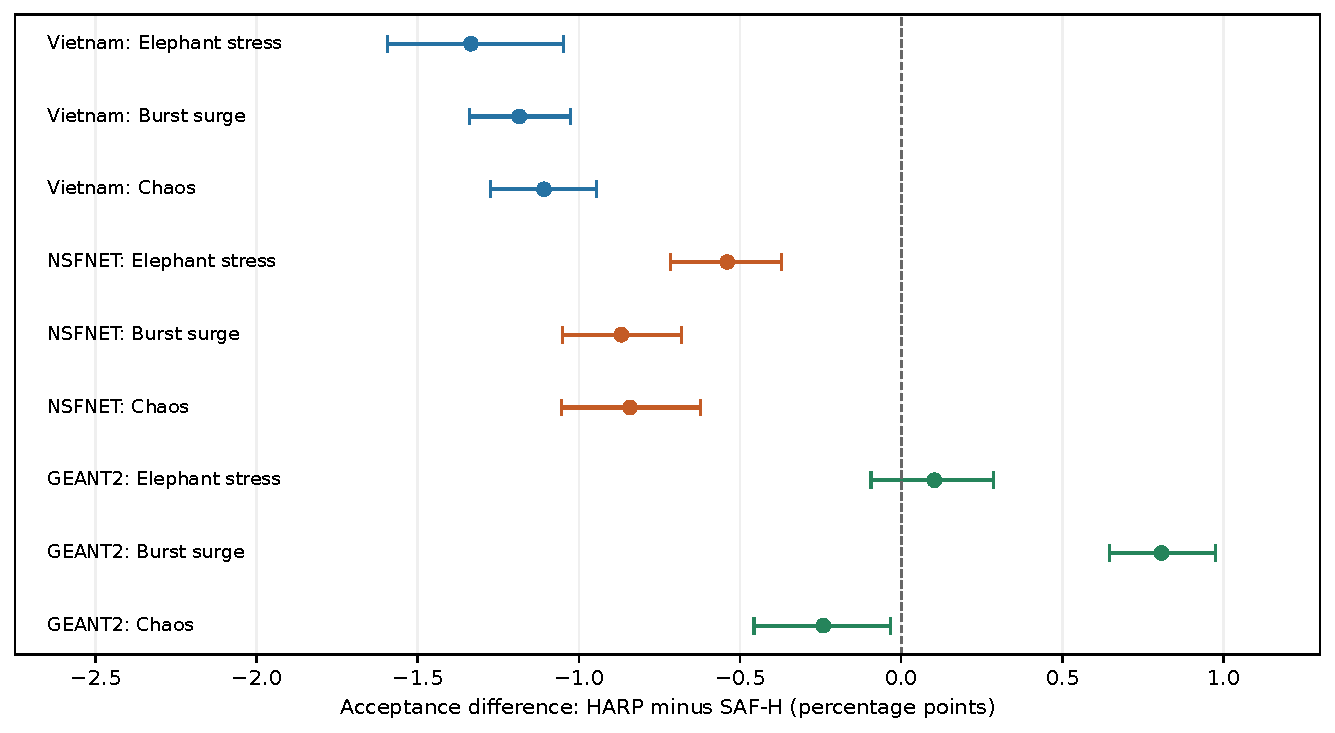
\includegraphics[width=0.94\textwidth]{figs/benchmark_paired_effects.pdf}
\caption{\newrev{Protected HARP minus SAF-H acceptance across three topologies and three stress workloads. Points show mean paired seed-level differences; horizontal intervals are percentile-bootstrap 95\% confidence intervals from paired seed-level trials. Positive values favor HARP. Holm-adjusted tests across all nine conditions are reported in main-manuscript Table~3.}}
\label{fig:benchmark_effects}
\end{figure*}

\begin{figure*}[p]
\centering
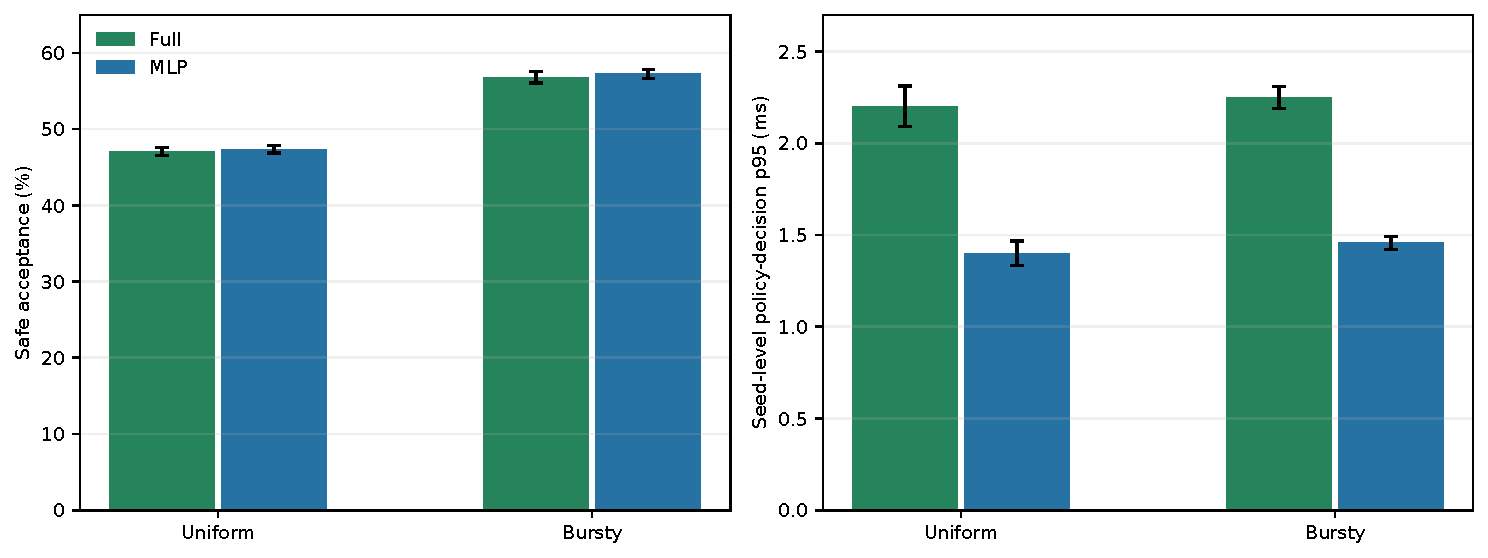
\includegraphics[width=0.94\textwidth]{figs/ablation_compute_cost.pdf}
\caption{\newrev{Acceptance and measured computation cost of Full and MLP ablation checkpoints on Vietnam. Bars show means and error bars show sample SD across 20 evaluation seeds. The right panel aggregates the per-seed P95 interval including normalization, inference, and simulator stepping; it excludes external controller actuation.}}
\label{fig:ablation_cost}
\end{figure*}

\begin{figure*}[p]
\centering
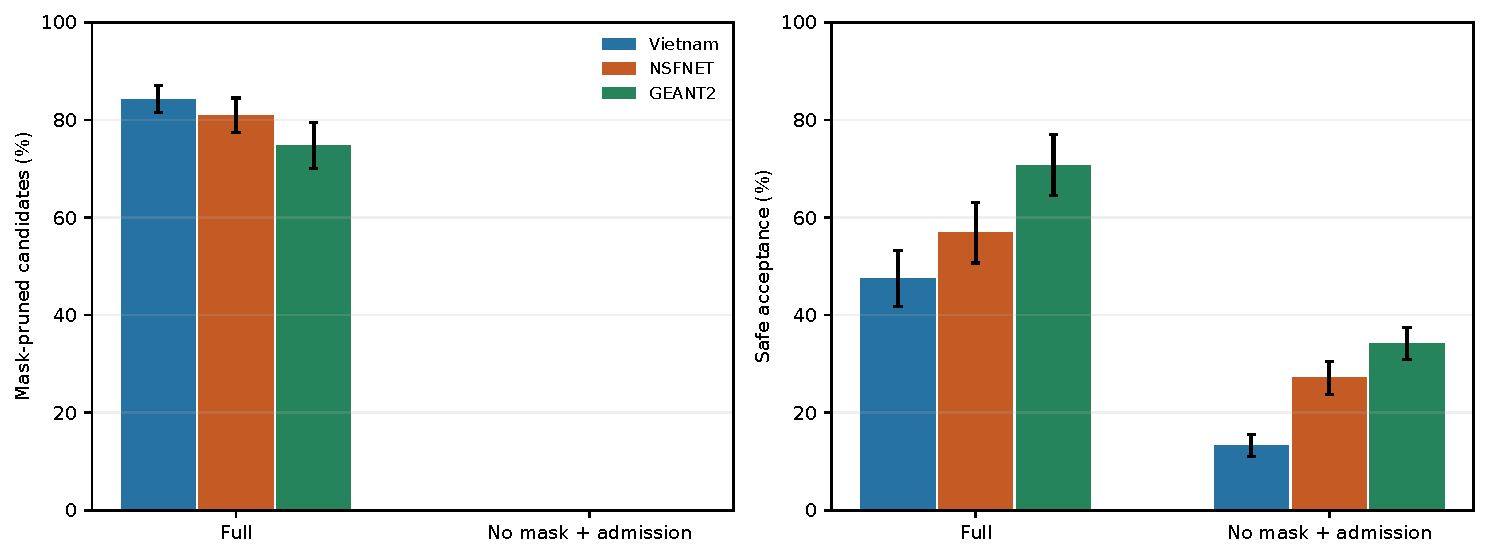
\includegraphics[width=0.94\textwidth]{figs/ablation_mask_admission.pdf}
\caption{\newrev{Candidate pruning and safe acceptance for Full and NoMask ablation variants with runtime admission enabled. Bars summarize 80 seed--workload cells per topology; error bars are sample SD across those cells. All six protected configurations recorded zero admitted hard violations. Distinct checkpoints and resulting state trajectories limit causal attribution to masking alone.}}
\label{fig:ablation_pruning}
\end{figure*}

% Inlined from evidence/load_sweep/mentor_b2_load_sweep_21.tex
\begin{table*}[p]
\centering
\color{revisiongreen}\small
\begin{tabular}{llrrrrrr}
\toprule
Topology & Intensity & $\Delta$ (pp) & 95\% CI & $p$ & $r_{rb}$ & $n_{eff}$ & $p_{Holm}$ \\
\midrule
VIETNAM & 0.2 & 0.000 & [0.000, 0.000] & 1 & -- & 0 & 1 \\
VIETNAM & 0.4 & 0.004 & [0.000, 0.012] & 1 & 1.000 & 1 & 1 \\
VIETNAM & 0.6 & 0.019 & [0.006, 0.038] & 0.0625 & 1.000 & 5 & 0.562 \\
VIETNAM & 0.8 & 0.401 & [0.353, 0.450] & 1.91e-06 & 1.000 & 20 & 4.01e-05 \\
VIETNAM & 1.0 & 1.213 & [1.132, 1.297] & 1.91e-06 & 1.000 & 20 & 4.01e-05 \\
VIETNAM & 1.2 & 2.515 & [2.415, 2.618] & 1.91e-06 & 1.000 & 20 & 4.01e-05 \\
VIETNAM & 1.5 & 2.402 & [2.278, 2.523] & 1.91e-06 & 1.000 & 20 & 4.01e-05 \\
NSFNET & 0.2 & 0.000 & [0.000, 0.000] & 1 & -- & 0 & 1 \\
NSFNET & 0.4 & 0.000 & [0.000, 0.000] & 1 & -- & 0 & 1 \\
NSFNET & 0.6 & 0.014 & [0.003, 0.028] & 0.125 & 1.000 & 4 & 1 \\
NSFNET & 0.8 & 0.253 & [0.201, 0.307] & 1.91e-06 & 1.000 & 20 & 4.01e-05 \\
NSFNET & 1.0 & 1.127 & [1.057, 1.190] & 1.91e-06 & 1.000 & 20 & 4.01e-05 \\
NSFNET & 1.2 & 3.213 & [3.070, 3.357] & 1.91e-06 & 1.000 & 20 & 4.01e-05 \\
NSFNET & 1.5 & 2.697 & [2.607, 2.802] & 1.91e-06 & 1.000 & 20 & 4.01e-05 \\
GEANT2 & 0.2 & 0.000 & [0.000, 0.000] & 1 & -- & 0 & 1 \\
GEANT2 & 0.4 & 0.000 & [0.000, 0.000] & 1 & -- & 0 & 1 \\
GEANT2 & 0.6 & 0.006 & [0.000, 0.014] & 0.5 & 1.000 & 2 & 1 \\
GEANT2 & 0.8 & 0.120 & [0.089, 0.154] & 3.81e-06 & 1.000 & 19 & 4.01e-05 \\
GEANT2 & 1.0 & 0.985 & [0.928, 1.040] & 1.91e-06 & 1.000 & 20 & 4.01e-05 \\
GEANT2 & 1.2 & 3.680 & [3.585, 3.770] & 1.91e-06 & 1.000 & 20 & 4.01e-05 \\
GEANT2 & 1.5 & 3.303 & [3.205, 3.403] & 1.91e-06 & 1.000 & 20 & 4.01e-05 \\
\bottomrule
\end{tabular}
\caption{Paired HARP--SAF-H safe-acceptance differences in the refreshed-model load sweep. $\Delta$ is the matched-seed mean; CI is a 20,000-resample paired percentile-bootstrap 95\% interval. $p$ is the exact two-sided Wilcoxon signed-rank test after dropping zeros and averaging tied absolute ranks; Holm correction covers all 21 topology--intensity tests.}
\label{tab:load_sweep_paired_statistics}
\end{table*}

% Inlined from evidence/load_sweep/mentor_d1_unprotected_load_sweep.tex
\begin{table*}[p]
\centering
\color{revisiongreen}\small
\begin{tabular}{llrrrrr}
\toprule
Intensity & Policy & CPU & RAM & BW & MSD & Any hard violation \\
\midrule
0.2 & Greedy & 0.000\textsuperscript{$\pm$0.000} & 0.000\textsuperscript{$\pm$0.000} & 0.000\textsuperscript{$\pm$0.000} & 0.378\textsuperscript{$\pm$0.201} & 0.378\textsuperscript{$\pm$0.201} \\
0.2 & DAI & 0.000\textsuperscript{$\pm$0.000} & 0.000\textsuperscript{$\pm$0.000} & 0.000\textsuperscript{$\pm$0.000} & 0.748\textsuperscript{$\pm$0.310} & 0.748\textsuperscript{$\pm$0.310} \\
0.2 & SAF-H & 0.000\textsuperscript{$\pm$0.000} & 0.000\textsuperscript{$\pm$0.000} & 0.000\textsuperscript{$\pm$0.000} & 0.865\textsuperscript{$\pm$0.334} & 0.865\textsuperscript{$\pm$0.334} \\
0.2 & HARP & 2.180\textsuperscript{$\pm$0.662} & 0.158\textsuperscript{$\pm$0.214} & 0.000\textsuperscript{$\pm$0.000} & 0.000\textsuperscript{$\pm$0.000} & 2.180\textsuperscript{$\pm$0.662} \\
0.4 & Greedy & 0.004\textsuperscript{$\pm$0.018} & 0.000\textsuperscript{$\pm$0.000} & 0.000\textsuperscript{$\pm$0.000} & 0.368\textsuperscript{$\pm$0.139} & 0.372\textsuperscript{$\pm$0.134} \\
0.4 & DAI & 0.004\textsuperscript{$\pm$0.018} & 0.000\textsuperscript{$\pm$0.000} & 0.000\textsuperscript{$\pm$0.000} & 0.687\textsuperscript{$\pm$0.198} & 0.692\textsuperscript{$\pm$0.201} \\
0.4 & SAF-H & 0.004\textsuperscript{$\pm$0.018} & 0.000\textsuperscript{$\pm$0.000} & 0.000\textsuperscript{$\pm$0.000} & 0.728\textsuperscript{$\pm$0.208} & 0.732\textsuperscript{$\pm$0.210} \\
0.4 & HARP & 6.853\textsuperscript{$\pm$0.837} & 2.298\textsuperscript{$\pm$0.689} & 0.000\textsuperscript{$\pm$0.000} & 0.000\textsuperscript{$\pm$0.000} & 6.853\textsuperscript{$\pm$0.837} \\
0.6 & Greedy & 0.019\textsuperscript{$\pm$0.037} & 0.000\textsuperscript{$\pm$0.000} & 0.000\textsuperscript{$\pm$0.000} & 0.289\textsuperscript{$\pm$0.154} & 0.308\textsuperscript{$\pm$0.170} \\
0.6 & DAI & 0.019\textsuperscript{$\pm$0.037} & 0.000\textsuperscript{$\pm$0.000} & 0.000\textsuperscript{$\pm$0.000} & 0.698\textsuperscript{$\pm$0.153} & 0.715\textsuperscript{$\pm$0.158} \\
0.6 & SAF-H & 0.019\textsuperscript{$\pm$0.037} & 0.000\textsuperscript{$\pm$0.000} & 0.000\textsuperscript{$\pm$0.000} & 0.703\textsuperscript{$\pm$0.176} & 0.720\textsuperscript{$\pm$0.186} \\
0.6 & HARP & 14.058\textsuperscript{$\pm$1.448} & 6.322\textsuperscript{$\pm$1.205} & 0.000\textsuperscript{$\pm$0.000} & 0.022\textsuperscript{$\pm$0.028} & 14.080\textsuperscript{$\pm$1.445} \\
0.8 & Greedy & 0.508\textsuperscript{$\pm$0.152} & 0.002\textsuperscript{$\pm$0.009} & 0.000\textsuperscript{$\pm$0.000} & 0.351\textsuperscript{$\pm$0.109} & 0.845\textsuperscript{$\pm$0.185} \\
0.8 & DAI & 0.509\textsuperscript{$\pm$0.150} & 0.000\textsuperscript{$\pm$0.000} & 0.000\textsuperscript{$\pm$0.000} & 0.735\textsuperscript{$\pm$0.131} & 1.206\textsuperscript{$\pm$0.188} \\
0.8 & SAF-H & 0.506\textsuperscript{$\pm$0.146} & 0.000\textsuperscript{$\pm$0.000} & 0.000\textsuperscript{$\pm$0.000} & 0.756\textsuperscript{$\pm$0.145} & 1.229\textsuperscript{$\pm$0.235} \\
0.8 & HARP & 27.387\textsuperscript{$\pm$1.456} & 16.232\textsuperscript{$\pm$1.393} & 0.000\textsuperscript{$\pm$0.000} & 0.044\textsuperscript{$\pm$0.044} & 27.428\textsuperscript{$\pm$1.441} \\
1.0 & Greedy & 2.158\textsuperscript{$\pm$0.240} & 0.005\textsuperscript{$\pm$0.012} & 0.000\textsuperscript{$\pm$0.000} & 0.342\textsuperscript{$\pm$0.113} & 2.467\textsuperscript{$\pm$0.290} \\
1.0 & DAI & 2.158\textsuperscript{$\pm$0.240} & 0.005\textsuperscript{$\pm$0.012} & 0.000\textsuperscript{$\pm$0.000} & 0.707\textsuperscript{$\pm$0.150} & 2.765\textsuperscript{$\pm$0.239} \\
1.0 & SAF-H & 2.162\textsuperscript{$\pm$0.240} & 0.005\textsuperscript{$\pm$0.012} & 0.000\textsuperscript{$\pm$0.000} & 0.717\textsuperscript{$\pm$0.114} & 2.775\textsuperscript{$\pm$0.209} \\
1.0 & HARP & 41.292\textsuperscript{$\pm$2.354} & 31.202\textsuperscript{$\pm$2.239} & 0.000\textsuperscript{$\pm$0.000} & 0.047\textsuperscript{$\pm$0.035} & 41.338\textsuperscript{$\pm$2.362} \\
1.2 & Greedy & 13.998\textsuperscript{$\pm$0.688} & 0.557\textsuperscript{$\pm$0.092} & 0.000\textsuperscript{$\pm$0.000} & 0.345\textsuperscript{$\pm$0.111} & 14.173\textsuperscript{$\pm$0.702} \\
1.2 & DAI & 13.978\textsuperscript{$\pm$0.777} & 0.660\textsuperscript{$\pm$0.192} & 0.000\textsuperscript{$\pm$0.000} & 0.722\textsuperscript{$\pm$0.128} & 14.352\textsuperscript{$\pm$0.755} \\
1.2 & SAF-H & 14.010\textsuperscript{$\pm$0.669} & 0.555\textsuperscript{$\pm$0.094} & 0.000\textsuperscript{$\pm$0.000} & 0.638\textsuperscript{$\pm$0.119} & 14.330\textsuperscript{$\pm$0.660} \\
1.2 & HARP & 55.490\textsuperscript{$\pm$1.947} & 50.573\textsuperscript{$\pm$2.092} & 0.093\textsuperscript{$\pm$0.110} & 0.090\textsuperscript{$\pm$0.057} & 55.573\textsuperscript{$\pm$1.953} \\
1.5 & Greedy & 58.993\textsuperscript{$\pm$2.023} & 12.195\textsuperscript{$\pm$0.790} & 0.000\textsuperscript{$\pm$0.000} & 10.872\textsuperscript{$\pm$0.309} & 60.855\textsuperscript{$\pm$1.881} \\
1.5 & DAI & 47.770\textsuperscript{$\pm$0.977} & 21.058\textsuperscript{$\pm$0.786} & 0.000\textsuperscript{$\pm$0.000} & 23.242\textsuperscript{$\pm$0.808} & 53.555\textsuperscript{$\pm$0.775} \\
1.5 & SAF-H & 58.972\textsuperscript{$\pm$2.042} & 12.182\textsuperscript{$\pm$0.774} & 0.000\textsuperscript{$\pm$0.000} & 21.417\textsuperscript{$\pm$0.205} & 62.790\textsuperscript{$\pm$1.934} \\
1.5 & HARP & 94.538\textsuperscript{$\pm$0.955} & 94.497\textsuperscript{$\pm$0.966} & 84.240\textsuperscript{$\pm$2.771} & 0.275\textsuperscript{$\pm$0.095} & 94.793\textsuperscript{$\pm$0.920} \\
\bottomrule
\end{tabular}
\caption{Vietnam offered-intensity experiment with admission disabled. Rates are mean and sample SD in percent over 20 seeds. The denominator is all offered requests; violation categories can overlap.}
\label{tab:load_sweep_unprotected}
\end{table*}
\begin{table*}[p]
\centering
\color{revisiongreen}\small
\begin{tabular}{llrrrrr}
\toprule
Intensity & Policy & CPU & RAM & BW & MSD & Any hard violation \\
\midrule
0.2 & Greedy & 0.000\textsuperscript{$\pm$0.000} & 0.000\textsuperscript{$\pm$0.000} & 0.000\textsuperscript{$\pm$0.000} & 0.000\textsuperscript{$\pm$0.000} & 0.000\textsuperscript{$\pm$0.000} \\
0.2 & DAI & 0.000\textsuperscript{$\pm$0.000} & 0.000\textsuperscript{$\pm$0.000} & 0.000\textsuperscript{$\pm$0.000} & 0.000\textsuperscript{$\pm$0.000} & 0.000\textsuperscript{$\pm$0.000} \\
0.2 & SAF-H & 0.000\textsuperscript{$\pm$0.000} & 0.000\textsuperscript{$\pm$0.000} & 0.000\textsuperscript{$\pm$0.000} & 0.000\textsuperscript{$\pm$0.000} & 0.000\textsuperscript{$\pm$0.000} \\
0.2 & HARP & 14.152\textsuperscript{$\pm$1.814} & 5.559\textsuperscript{$\pm$1.339} & 0.000\textsuperscript{$\pm$0.000} & 0.000\textsuperscript{$\pm$0.000} & 14.152\textsuperscript{$\pm$1.814} \\
0.4 & Greedy & 0.000\textsuperscript{$\pm$0.000} & 0.000\textsuperscript{$\pm$0.000} & 0.000\textsuperscript{$\pm$0.000} & 0.000\textsuperscript{$\pm$0.000} & 0.000\textsuperscript{$\pm$0.000} \\
0.4 & DAI & 0.000\textsuperscript{$\pm$0.000} & 0.000\textsuperscript{$\pm$0.000} & 0.000\textsuperscript{$\pm$0.000} & 0.000\textsuperscript{$\pm$0.000} & 0.000\textsuperscript{$\pm$0.000} \\
0.4 & SAF-H & 0.000\textsuperscript{$\pm$0.000} & 0.000\textsuperscript{$\pm$0.000} & 0.000\textsuperscript{$\pm$0.000} & 0.000\textsuperscript{$\pm$0.000} & 0.000\textsuperscript{$\pm$0.000} \\
0.4 & HARP & 15.563\textsuperscript{$\pm$1.045} & 8.110\textsuperscript{$\pm$1.052} & 0.000\textsuperscript{$\pm$0.000} & 0.000\textsuperscript{$\pm$0.000} & 15.563\textsuperscript{$\pm$1.045} \\
0.6 & Greedy & 0.014\textsuperscript{$\pm$0.040} & 0.000\textsuperscript{$\pm$0.000} & 0.000\textsuperscript{$\pm$0.000} & 0.000\textsuperscript{$\pm$0.000} & 0.014\textsuperscript{$\pm$0.040} \\
0.6 & DAI & 0.019\textsuperscript{$\pm$0.045} & 0.000\textsuperscript{$\pm$0.000} & 0.000\textsuperscript{$\pm$0.000} & 0.000\textsuperscript{$\pm$0.000} & 0.019\textsuperscript{$\pm$0.045} \\
0.6 & SAF-H & 0.019\textsuperscript{$\pm$0.045} & 0.000\textsuperscript{$\pm$0.000} & 0.000\textsuperscript{$\pm$0.000} & 0.000\textsuperscript{$\pm$0.000} & 0.019\textsuperscript{$\pm$0.045} \\
0.6 & HARP & 25.150\textsuperscript{$\pm$2.933} & 8.493\textsuperscript{$\pm$1.116} & 0.000\textsuperscript{$\pm$0.000} & 0.000\textsuperscript{$\pm$0.000} & 25.150\textsuperscript{$\pm$2.933} \\
0.8 & Greedy & 0.330\textsuperscript{$\pm$0.081} & 0.000\textsuperscript{$\pm$0.000} & 0.000\textsuperscript{$\pm$0.000} & 0.000\textsuperscript{$\pm$0.000} & 0.330\textsuperscript{$\pm$0.081} \\
0.8 & DAI & 0.332\textsuperscript{$\pm$0.082} & 0.000\textsuperscript{$\pm$0.000} & 0.000\textsuperscript{$\pm$0.000} & 0.000\textsuperscript{$\pm$0.000} & 0.332\textsuperscript{$\pm$0.082} \\
0.8 & SAF-H & 0.330\textsuperscript{$\pm$0.080} & 0.000\textsuperscript{$\pm$0.000} & 0.000\textsuperscript{$\pm$0.000} & 0.000\textsuperscript{$\pm$0.000} & 0.330\textsuperscript{$\pm$0.080} \\
0.8 & HARP & 53.319\textsuperscript{$\pm$3.290} & 21.684\textsuperscript{$\pm$2.588} & 0.000\textsuperscript{$\pm$0.000} & 0.000\textsuperscript{$\pm$0.000} & 53.319\textsuperscript{$\pm$3.290} \\
1.0 & Greedy & 1.747\textsuperscript{$\pm$0.203} & 0.005\textsuperscript{$\pm$0.012} & 0.000\textsuperscript{$\pm$0.000} & 0.000\textsuperscript{$\pm$0.000} & 1.747\textsuperscript{$\pm$0.203} \\
1.0 & DAI & 1.742\textsuperscript{$\pm$0.201} & 0.005\textsuperscript{$\pm$0.012} & 0.000\textsuperscript{$\pm$0.000} & 0.000\textsuperscript{$\pm$0.000} & 1.742\textsuperscript{$\pm$0.201} \\
1.0 & SAF-H & 1.728\textsuperscript{$\pm$0.206} & 0.005\textsuperscript{$\pm$0.012} & 0.000\textsuperscript{$\pm$0.000} & 0.000\textsuperscript{$\pm$0.000} & 1.728\textsuperscript{$\pm$0.206} \\
1.0 & HARP & 69.373\textsuperscript{$\pm$2.461} & 44.325\textsuperscript{$\pm$3.262} & 0.000\textsuperscript{$\pm$0.000} & 0.000\textsuperscript{$\pm$0.000} & 69.373\textsuperscript{$\pm$2.461} \\
1.2 & Greedy & 12.332\textsuperscript{$\pm$0.552} & 0.368\textsuperscript{$\pm$0.091} & 0.000\textsuperscript{$\pm$0.000} & 0.000\textsuperscript{$\pm$0.000} & 12.332\textsuperscript{$\pm$0.552} \\
1.2 & DAI & 12.307\textsuperscript{$\pm$0.639} & 0.367\textsuperscript{$\pm$0.079} & 0.000\textsuperscript{$\pm$0.000} & 0.000\textsuperscript{$\pm$0.000} & 12.307\textsuperscript{$\pm$0.639} \\
1.2 & SAF-H & 12.288\textsuperscript{$\pm$0.627} & 0.365\textsuperscript{$\pm$0.097} & 0.000\textsuperscript{$\pm$0.000} & 0.000\textsuperscript{$\pm$0.000} & 12.288\textsuperscript{$\pm$0.627} \\
1.2 & HARP & 75.437\textsuperscript{$\pm$1.761} & 59.025\textsuperscript{$\pm$3.845} & 0.057\textsuperscript{$\pm$0.068} & 0.000\textsuperscript{$\pm$0.000} & 75.437\textsuperscript{$\pm$1.761} \\
1.5 & Greedy & 58.308\textsuperscript{$\pm$2.128} & 11.053\textsuperscript{$\pm$0.800} & 0.000\textsuperscript{$\pm$0.000} & 1.008\textsuperscript{$\pm$0.138} & 58.467\textsuperscript{$\pm$2.115} \\
1.5 & DAI & 47.147\textsuperscript{$\pm$1.406} & 19.627\textsuperscript{$\pm$1.506} & 0.000\textsuperscript{$\pm$0.000} & 3.110\textsuperscript{$\pm$0.491} & 47.725\textsuperscript{$\pm$1.418} \\
1.5 & SAF-H & 58.308\textsuperscript{$\pm$2.128} & 11.053\textsuperscript{$\pm$0.800} & 0.000\textsuperscript{$\pm$0.000} & 3.052\textsuperscript{$\pm$0.193} & 58.743\textsuperscript{$\pm$2.090} \\
1.5 & HARP & 81.085\textsuperscript{$\pm$3.878} & 73.348\textsuperscript{$\pm$6.122} & 5.948\textsuperscript{$\pm$2.203} & 3.407\textsuperscript{$\pm$0.063} & 81.428\textsuperscript{$\pm$3.807} \\
\bottomrule
\end{tabular}
\caption{NSFNET offered-intensity experiment with admission disabled. Rates are mean and sample SD in percent over 20 seeds. The denominator is all offered requests; violation categories can overlap.}
\label{tab:load_sweep_unprotected_nsfnet}
\end{table*}
\begin{table*}[p]
\centering
\color{revisiongreen}\small
\begin{tabular}{llrrrrr}
\toprule
Intensity & Policy & CPU & RAM & BW & MSD & Any hard violation \\
\midrule
0.2 & Greedy & 0.000\textsuperscript{$\pm$0.000} & 0.000\textsuperscript{$\pm$0.000} & 0.000\textsuperscript{$\pm$0.000} & 0.000\textsuperscript{$\pm$0.000} & 0.000\textsuperscript{$\pm$0.000} \\
0.2 & DAI & 0.000\textsuperscript{$\pm$0.000} & 0.000\textsuperscript{$\pm$0.000} & 0.000\textsuperscript{$\pm$0.000} & 0.000\textsuperscript{$\pm$0.000} & 0.000\textsuperscript{$\pm$0.000} \\
0.2 & SAF-H & 0.000\textsuperscript{$\pm$0.000} & 0.000\textsuperscript{$\pm$0.000} & 0.000\textsuperscript{$\pm$0.000} & 0.000\textsuperscript{$\pm$0.000} & 0.000\textsuperscript{$\pm$0.000} \\
0.2 & HARP & 22.580\textsuperscript{$\pm$5.343} & 5.397\textsuperscript{$\pm$2.950} & 0.000\textsuperscript{$\pm$0.000} & 0.000\textsuperscript{$\pm$0.000} & 22.580\textsuperscript{$\pm$5.343} \\
0.4 & Greedy & 0.000\textsuperscript{$\pm$0.000} & 0.000\textsuperscript{$\pm$0.000} & 0.000\textsuperscript{$\pm$0.000} & 0.000\textsuperscript{$\pm$0.000} & 0.000\textsuperscript{$\pm$0.000} \\
0.4 & DAI & 0.000\textsuperscript{$\pm$0.000} & 0.000\textsuperscript{$\pm$0.000} & 0.000\textsuperscript{$\pm$0.000} & 0.000\textsuperscript{$\pm$0.000} & 0.000\textsuperscript{$\pm$0.000} \\
0.4 & SAF-H & 0.000\textsuperscript{$\pm$0.000} & 0.000\textsuperscript{$\pm$0.000} & 0.000\textsuperscript{$\pm$0.000} & 0.000\textsuperscript{$\pm$0.000} & 0.000\textsuperscript{$\pm$0.000} \\
0.4 & HARP & 36.704\textsuperscript{$\pm$4.185} & 16.846\textsuperscript{$\pm$2.107} & 0.000\textsuperscript{$\pm$0.000} & 0.000\textsuperscript{$\pm$0.000} & 36.713\textsuperscript{$\pm$4.179} \\
0.6 & Greedy & 0.006\textsuperscript{$\pm$0.017} & 0.000\textsuperscript{$\pm$0.000} & 0.000\textsuperscript{$\pm$0.000} & 0.000\textsuperscript{$\pm$0.000} & 0.006\textsuperscript{$\pm$0.017} \\
0.6 & DAI & 0.006\textsuperscript{$\pm$0.017} & 0.000\textsuperscript{$\pm$0.000} & 0.000\textsuperscript{$\pm$0.000} & 0.000\textsuperscript{$\pm$0.000} & 0.006\textsuperscript{$\pm$0.017} \\
0.6 & SAF-H & 0.006\textsuperscript{$\pm$0.017} & 0.000\textsuperscript{$\pm$0.000} & 0.000\textsuperscript{$\pm$0.000} & 0.000\textsuperscript{$\pm$0.000} & 0.006\textsuperscript{$\pm$0.017} \\
0.6 & HARP & 78.464\textsuperscript{$\pm$2.844} & 46.151\textsuperscript{$\pm$3.730} & 0.000\textsuperscript{$\pm$0.000} & 0.000\textsuperscript{$\pm$0.000} & 78.464\textsuperscript{$\pm$2.844} \\
0.8 & Greedy & 0.112\textsuperscript{$\pm$0.070} & 0.000\textsuperscript{$\pm$0.000} & 0.000\textsuperscript{$\pm$0.000} & 0.000\textsuperscript{$\pm$0.000} & 0.112\textsuperscript{$\pm$0.070} \\
0.8 & DAI & 0.110\textsuperscript{$\pm$0.069} & 0.000\textsuperscript{$\pm$0.000} & 0.000\textsuperscript{$\pm$0.000} & 0.000\textsuperscript{$\pm$0.000} & 0.110\textsuperscript{$\pm$0.069} \\
0.8 & SAF-H & 0.112\textsuperscript{$\pm$0.072} & 0.000\textsuperscript{$\pm$0.000} & 0.000\textsuperscript{$\pm$0.000} & 0.000\textsuperscript{$\pm$0.000} & 0.112\textsuperscript{$\pm$0.072} \\
0.8 & HARP & 88.073\textsuperscript{$\pm$0.769} & 80.184\textsuperscript{$\pm$2.039} & 0.037\textsuperscript{$\pm$0.059} & 0.000\textsuperscript{$\pm$0.000} & 88.073\textsuperscript{$\pm$0.769} \\
1.0 & Greedy & 1.248\textsuperscript{$\pm$0.160} & 0.003\textsuperscript{$\pm$0.010} & 0.000\textsuperscript{$\pm$0.000} & 0.000\textsuperscript{$\pm$0.000} & 1.248\textsuperscript{$\pm$0.160} \\
1.0 & DAI & 1.242\textsuperscript{$\pm$0.150} & 0.002\textsuperscript{$\pm$0.007} & 0.000\textsuperscript{$\pm$0.000} & 0.000\textsuperscript{$\pm$0.000} & 1.242\textsuperscript{$\pm$0.150} \\
1.0 & SAF-H & 1.247\textsuperscript{$\pm$0.159} & 0.003\textsuperscript{$\pm$0.010} & 0.000\textsuperscript{$\pm$0.000} & 0.000\textsuperscript{$\pm$0.000} & 1.247\textsuperscript{$\pm$0.159} \\
1.0 & HARP & 90.202\textsuperscript{$\pm$0.813} & 89.118\textsuperscript{$\pm$1.011} & 0.782\textsuperscript{$\pm$0.385} & 0.000\textsuperscript{$\pm$0.000} & 90.202\textsuperscript{$\pm$0.813} \\
1.2 & Greedy & 11.328\textsuperscript{$\pm$0.563} & 0.267\textsuperscript{$\pm$0.073} & 0.000\textsuperscript{$\pm$0.000} & 0.000\textsuperscript{$\pm$0.000} & 11.328\textsuperscript{$\pm$0.563} \\
1.2 & DAI & 11.317\textsuperscript{$\pm$0.562} & 0.267\textsuperscript{$\pm$0.073} & 0.000\textsuperscript{$\pm$0.000} & 0.000\textsuperscript{$\pm$0.000} & 11.317\textsuperscript{$\pm$0.562} \\
1.2 & SAF-H & 11.313\textsuperscript{$\pm$0.560} & 0.263\textsuperscript{$\pm$0.076} & 0.000\textsuperscript{$\pm$0.000} & 0.000\textsuperscript{$\pm$0.000} & 11.313\textsuperscript{$\pm$0.560} \\
1.2 & HARP & 94.368\textsuperscript{$\pm$0.550} & 93.517\textsuperscript{$\pm$0.528} & 8.848\textsuperscript{$\pm$0.645} & 0.000\textsuperscript{$\pm$0.000} & 94.368\textsuperscript{$\pm$0.550} \\
1.5 & Greedy & 57.227\textsuperscript{$\pm$2.820} & 10.035\textsuperscript{$\pm$0.827} & 0.000\textsuperscript{$\pm$0.000} & 4.955\textsuperscript{$\pm$0.234} & 58.050\textsuperscript{$\pm$2.759} \\
1.5 & DAI & 45.788\textsuperscript{$\pm$1.696} & 16.995\textsuperscript{$\pm$1.430} & 0.012\textsuperscript{$\pm$0.038} & 4.270\textsuperscript{$\pm$0.616} & 46.715\textsuperscript{$\pm$1.712} \\
1.5 & SAF-H & 57.190\textsuperscript{$\pm$2.915} & 10.037\textsuperscript{$\pm$0.771} & 0.000\textsuperscript{$\pm$0.000} & 3.970\textsuperscript{$\pm$0.249} & 57.817\textsuperscript{$\pm$2.856} \\
1.5 & HARP & 97.005\textsuperscript{$\pm$0.663} & 93.413\textsuperscript{$\pm$0.980} & 58.997\textsuperscript{$\pm$2.818} & 0.000\textsuperscript{$\pm$0.000} & 97.005\textsuperscript{$\pm$0.663} \\
\bottomrule
\end{tabular}
\caption{GEANT2 offered-intensity experiment with admission disabled. Rates are mean and sample SD in percent over 20 seeds. The denominator is all offered requests; violation categories can overlap.}
\label{tab:load_sweep_unprotected_geant2}
\end{table*}

\begin{table*}[p]
\centering
\caption{Unprotected stress benchmark: mean admitted modeled violations across 20 seeds (percent of offered requests). CPU, RAM, bandwidth, and MSD categories may overlap; the union counts each request once.}
\label{tab:unprotected_stress}
\scriptsize
\begin{tabular}{lllrrrrr}
\toprule
Network & Profile & Policy & CPU & RAM & BW & MSD & Union \\
\midrule
% Inlined from evidence/mentor_completion_20261121/unprotected_stress_rows.tex
Vietnam & Elephant stress & Greedy & 98.772 & 96.523 & 55.792 & 2.942 & 98.795 \\
Vietnam & Elephant stress & DAI & 91.975 & 84.662 & 62.062 & 6.950 & 92.178 \\
Vietnam & Elephant stress & SAF-H & 98.772 & 96.522 & 0.000 & 6.125 & 98.847 \\
Vietnam & Elephant stress & CSPF & 99.750 & 99.280 & 98.690 & 0.000 & 99.750 \\
Vietnam & Elephant stress & HARP & 87.483 & 80.277 & 67.965 & 0.800 & 87.525 \\
Vietnam & Burst surge & Greedy & 98.100 & 96.558 & 5.792 & 0.342 & 98.100 \\
Vietnam & Burst surge & DAI & 86.498 & 76.925 & 34.188 & 0.732 & 86.528 \\
Vietnam & Burst surge & SAF-H & 98.100 & 96.558 & 0.000 & 0.662 & 98.100 \\
Vietnam & Burst surge & CSPF & 99.600 & 99.233 & 98.067 & 0.000 & 99.600 \\
Vietnam & Burst surge & HARP & 80.650 & 77.833 & 71.438 & 0.045 & 80.732 \\
Vietnam & Chaos & Greedy & 98.690 & 97.067 & 55.608 & 1.708 & 98.693 \\
Vietnam & Chaos & DAI & 91.617 & 84.597 & 60.330 & 3.758 & 91.705 \\
Vietnam & Chaos & SAF-H & 98.690 & 97.067 & 0.000 & 3.322 & 98.735 \\
Vietnam & Chaos & CSPF & 99.730 & 99.375 & 98.628 & 0.000 & 99.730 \\
Vietnam & Chaos & HARP & 87.018 & 80.765 & 73.787 & 0.080 & 87.082 \\
NSFNET & Elephant stress & Greedy & 98.277 & 94.738 & 43.827 & 0.000 & 98.277 \\
NSFNET & Elephant stress & DAI & 88.365 & 77.960 & 53.842 & 0.323 & 88.367 \\
NSFNET & Elephant stress & SAF-H & 98.277 & 94.738 & 0.000 & 0.288 & 98.277 \\
NSFNET & Elephant stress & CSPF & 99.750 & 99.280 & 98.690 & 0.000 & 99.750 \\
NSFNET & Elephant stress & HARP & 93.522 & 85.062 & 57.158 & 0.003 & 93.532 \\
NSFNET & Burst surge & Greedy & 97.080 & 94.763 & 0.000 & 0.000 & 97.080 \\
NSFNET & Burst surge & DAI & 80.615 & 67.115 & 23.485 & 0.000 & 80.617 \\
NSFNET & Burst surge & SAF-H & 97.080 & 94.763 & 0.000 & 0.000 & 97.080 \\
NSFNET & Burst surge & CSPF & 99.600 & 99.233 & 98.067 & 0.000 & 99.600 \\
NSFNET & Burst surge & HARP & 92.140 & 88.757 & 38.045 & 0.000 & 92.142 \\
NSFNET & Chaos & Greedy & 98.238 & 95.530 & 39.647 & 0.000 & 98.238 \\
NSFNET & Chaos & DAI & 87.928 & 77.918 & 49.657 & 0.042 & 87.928 \\
NSFNET & Chaos & SAF-H & 98.238 & 95.530 & 0.000 & 0.032 & 98.238 \\
NSFNET & Chaos & CSPF & 99.730 & 99.375 & 98.628 & 0.000 & 99.730 \\
NSFNET & Chaos & HARP & 93.600 & 85.847 & 55.412 & 0.000 & 93.600 \\
GEANT2 & Elephant stress & Greedy & 97.207 & 71.468 & 0.000 & 0.905 & 97.237 \\
GEANT2 & Elephant stress & DAI & 80.805 & 63.572 & 37.043 & 0.742 & 80.837 \\
GEANT2 & Elephant stress & SAF-H & 97.207 & 71.508 & 0.000 & 0.690 & 97.220 \\
GEANT2 & Elephant stress & CSPF & 99.750 & 99.280 & 98.690 & 0.000 & 99.750 \\
GEANT2 & Elephant stress & HARP & 92.535 & 83.725 & 50.873 & 0.000 & 92.535 \\
GEANT2 & Burst surge & Greedy & 94.453 & 73.043 & 0.000 & 0.000 & 94.453 \\
GEANT2 & Burst surge & DAI & 67.055 & 45.090 & 7.442 & 0.000 & 67.060 \\
GEANT2 & Burst surge & SAF-H & 94.453 & 73.008 & 0.000 & 0.000 & 94.453 \\
GEANT2 & Burst surge & CSPF & 99.600 & 99.233 & 98.067 & 0.000 & 99.600 \\
GEANT2 & Burst surge & HARP & 95.055 & 94.422 & 56.653 & 0.000 & 95.057 \\
GEANT2 & Chaos & Greedy & 97.092 & 84.120 & 0.000 & 0.138 & 97.092 \\
GEANT2 & Chaos & DAI & 79.562 & 62.637 & 33.943 & 0.133 & 79.563 \\
GEANT2 & Chaos & SAF-H & 97.092 & 84.063 & 0.000 & 0.128 & 97.092 \\
GEANT2 & Chaos & CSPF & 99.730 & 99.375 & 98.628 & 0.000 & 99.730 \\
GEANT2 & Chaos & HARP & 96.038 & 94.972 & 80.345 & 0.000 & 96.038 \\

\bottomrule
\end{tabular}
\end{table*}


\begin{table*}[p]
\centering
\caption{\newrev{Simulated service quality for the admitted requests of each policy. Each cell averages 20 seed-level measurements. The policies may admit different request populations.}}
\label{tab:stress_qos}
{\color{revisiongreen}
\begin{tabular}{llrrrr}
\toprule
& & \multicolumn{2}{c}{HARP} & \multicolumn{2}{c}{SAF-H} \\
\cmidrule(lr){3-4}\cmidrule(lr){5-6}
Topology & Workload & Latency (ms) & SLA violation (\%) & Latency (ms) & SLA violation (\%) \\
\midrule
% Inlined from generated/qos_rows.tex
Vietnam & Elephant stress & 5.47 & 0.05 & 0.56 & 0.00 \\
Vietnam & Burst surge & 5.25 & 0.00 & 0.62 & 0.00 \\
Vietnam & Chaos & 5.53 & 0.02 & 0.56 & 0.00 \\
NSFNET & Elephant stress & 7.05 & 0.04 & 0.45 & 0.00 \\
NSFNET & Burst surge & 7.39 & 0.06 & 0.47 & 0.00 \\
NSFNET & Chaos & 6.78 & 0.02 & 0.46 & 0.00 \\
GEANT2 & Elephant stress & 7.17 & 0.21 & 0.34 & 0.00 \\
GEANT2 & Burst surge & 7.16 & 0.12 & 0.32 & 0.00 \\
GEANT2 & Chaos & 7.34 & 0.15 & 0.34 & 0.00 \\

\bottomrule
\end{tabular}
}
\end{table*}

\begin{table*}[p]
\centering
\caption{\newrev{Paired HARP minus SAF-H safe-acceptance differences in the fixed-profile arrival-rate experiment (percentage points; 20 matched seeds). Intervals are paired percentile-bootstrap 95\% CIs; $p_H$ is the exact signed-rank p-value after Holm correction over 15 topology--rate cells.}}
\label{tab:arrival_rate_paired_statistics}
\scriptsize
\begin{tabular}{llrrrrr}
\toprule
Topology & Arrival probability & Mean difference & 95\% CI & $p$ & $p_H$ \\
\midrule
% Inlined from generated/arrival_rate_paired_rows.tex
VIETNAM & 0.2 & 2.221 & [1.865, 2.574] & 1.91e-06 & 2.86e-05 \\
VIETNAM & 0.4 & 0.544 & [0.328, 0.758] & 0.000168 & 0.000504 \\
VIETNAM & 0.6 & -0.950 & [-1.164, -0.744] & 1.91e-06 & 2.86e-05 \\
VIETNAM & 0.8 & -1.593 & [-1.810, -1.387] & 1.91e-06 & 2.86e-05 \\
VIETNAM & 1.0 & -1.185 & [-1.340, -1.023] & 1.91e-06 & 2.86e-05 \\
NSFNET & 0.2 & 2.064 & [1.837, 2.294] & 1.91e-06 & 2.86e-05 \\
NSFNET & 0.4 & 1.998 & [1.800, 2.176] & 1.91e-06 & 2.86e-05 \\
NSFNET & 0.6 & 0.476 & [0.307, 0.637] & 0.000105 & 0.00042 \\
NSFNET & 0.8 & -0.321 & [-0.539, -0.105] & 0.0159 & 0.0319 \\
NSFNET & 1.0 & -0.868 & [-1.048, -0.685] & 1.91e-06 & 2.86e-05 \\
GEANT2 & 0.2 & 0.017 & [0.000, 0.043] & 0.5 & 0.5 \\
GEANT2 & 0.4 & 3.067 & [2.916, 3.220] & 1.91e-06 & 2.86e-05 \\
GEANT2 & 0.6 & 2.935 & [2.740, 3.125] & 1.91e-06 & 2.86e-05 \\
GEANT2 & 0.8 & 1.612 & [1.476, 1.760] & 1.91e-06 & 2.86e-05 \\
GEANT2 & 1.0 & 0.808 & [0.645, 0.977] & 3.81e-06 & 2.86e-05 \\

\bottomrule
\end{tabular}
\end{table*}
\begin{table*}[p]
\centering
\caption{\newrev{Independent HARP training on Vietnam at the nominal 2M-transition budget. Each model is evaluated on 20 matched Bursty stress seeds; acceptance is in percent, and SD is across evaluation seeds. Training seeds and evaluation seeds are separate experimental factors.}}
\label{tab:independent_training}
{\color{revisiongreen}
\begin{tabular}{rrrr}
\toprule
Training seed & Saved transitions & Mean safe acceptance (\%) & Evaluation SD (pp) \\
\midrule
% Inlined from generated/independent_training_rows.tex
42 & 2,002,944 & 57.657 & 0.679 \\
7 & 2,002,944 & 57.375 & 0.601 \\
2024 & 2,002,944 & 57.633 & 0.504 \\

\bottomrule
\end{tabular}}
\end{table*}
\clearpage
\endgroup

\begin{table*}[t]
\centering
\caption{\newrev{Request-correlated end-to-end HIL campaigns. Timed rows give P50 / P95 / P99 over steered requests, except the admission API row, which covers all offered requests. Probe rows count the in-campaign probe; re-probes after the firewall correction are reported in the text.}}
\label{tab:hil_e2e_detailed}
{\color{revisiongreen}
\small
% Inlined from generated/table_hil_e2e.tex
\begin{tabular}{@{}lrr@{}}
\toprule
Metric (P50 / P95 / P99 where timed) & Corrected checkpoint & Pre-correction checkpoint \\
\midrule
Offered requests & 398 & 148 \\
Admitted (HTTP 200) & 69 & 31 \\
Steering confirmed by controller & 69 & 27 \\
Installed rules read back on every path switch & 69 & 27 \\
Rejected: requested depth $\neq$ materialized depth & 231 & 105 \\
Rejected: path exceeds switch MSD profile & 6 & 0 \\
\newrev{Rejected: ingress equals placement} & \newrev{43} & \newrev{12} \\
\newrev{Rejected: no feasible resilience pair} & \newrev{49} & \newrev{0} \\
\newrev{All rejected requests} & \newrev{329} & \newrev{117} \\
\newrev{Admitted with actuation warning} & \newrev{0} & \newrev{4} \\
\newrev{Initial / final active VNFs} & \newrev{39 / 51} & \newrev{---} \\
\newrev{Deployments without replacement} & \newrev{12} & \newrev{--} \\
Probes with 20/20 packets at the VNF & 64 / 69 & 27 / 27 \\
Probe packets received / sent & 1,280 / 1,380 & 540 / 540 \\
Migrations; make-before-break order held & 57; 57 & 23; 23 \\
Migrations completed (old VNF absence confirmed) & 57 & 19 \\
Admission API response (s) & 0.147 / 0.243 / 0.449 & 0.127 / 0.185 / 0.220 \\
Tekton PipelineRun duration (s) & 34 / 45 / 83 & 32 / 36 / 37 \\
Deployment start to Pod Ready (s) & 20.4 / 28.8 / 32.0 & 17.4 / 24.2 / 24.2 \\
Rule installation and readback confirmation (s) & 0.54 / 0.80 / 1.09 & 0.55 / 1.42 / 2.16 \\
Submission to steering confirmation (s) & 23.2 / 31.6 / 35.1 & 20.8 / 27.4 / 27.6 \\
Probe RTT through SRv6, per-probe median (ms) & 3.3 / 9.7 / 10.6 & 4.1 / 10.6 / 10.8 \\
\bottomrule
\end{tabular}

}
\end{table*}

\begin{table*}[p]
\centering
\caption{Full BMv2 over-MSD trials, including the per-switch path profiles. Isolated rows aggregate three 100-packet trials per mode; live rows use 50 packets per depth.}
\label{tab:hil_msd_detailed}
{\scriptsize% Inlined from generated/table_hil_msd_detailed.tex
\begin{tabular}{@{}llrlrrl@{}}
\toprule
Experiment & Path (per-switch MSD) & Depth & Admission & Rules & Rx / Tx & Counter \\
\midrule
Isolated, protected & s2-s1-s6-s7 (10,10,8,4) & 4 & admit & 4 & 300 / 300 & 0 \\
Isolated, bypass & s2-s1-s6-s7 (10,10,8,4) & 4 & bypassed & 4 & 300 / 300 & 0 \\
Isolated, protected & s2-s1-s6-s7-s8 (10,10,8,4,5) & 5 & reject & 0 & 0 / 0 & 0 \\
Isolated, bypass & s2-s1-s6-s7-s8 (10,10,8,4,5) & 5 & bypassed & 5 & 0 / 300 & s7 +300 \\
\midrule
Live, admitted path & s2-s1-s6-s5 (10,10,8,4) & 4 & at admitted depth & installed & 50 / 50 & 0 \\
Live, admitted path & s2-s1-s6-s5 (10,10,8,4) & 7 & bypassed & installed & 0 / 50 & s5 +50 \\
Live, admitted path & s2-s1-s6-s5 (10,10,8,4) & 9 & bypassed & installed & 0 / 50 & s6 +50 \\
Live, admitted path & s2-s1-s6-s5 (10,10,8,4) & 11 & bypassed & installed & 0 / 50 & s2 +50 \\
\bottomrule
\end{tabular}
}
\end{table*}
\begin{table*}[p]
\centering
\caption{\newrev{Audited admission-validation overhead from retained benchmark logs. Left: synthetic 25/50/100-node Burst-surge stress, 20 matched seeds. Right: the named-substrate occupancy protocol at intensity 1.0, 20 seeds. All cells are mean\textsuperscript{$\pm$SD} of seed-level P95 (ms); validation covers predicates, excluding resource mutation and external reservation. These protocols do not provide a crossed synthetic-size/occupancy experiment.}}
\label{tab:safety_validation_scaling}
\begin{minipage}[t]{0.49\textwidth}
{\color{revisiongreen}
\footnotesize
\setlength{\tabcolsep}{4pt}
\resizebox{\columnwidth}{!}{%
\begin{tabular}{lrr}
\toprule
Component P95 (ms) & HARP & SAF-H \\
\midrule
\multicolumn{3}{l}{\textit{25 nodes}} \\
Normalization & 0.067\textsuperscript{$\pm$0.016} & --- \\
Candidate construction & 0.550\textsuperscript{$\pm$0.070} & 0.503\textsuperscript{$\pm$0.026} \\
Inference / selection & 3.948\textsuperscript{$\pm$0.560} & 1.121\textsuperscript{$\pm$0.080} \\
Admission validation & 0.0058\textsuperscript{$\pm$0.0006} & 0.0024\textsuperscript{$\pm$0.0001} \\
Total decision & 5.378\textsuperscript{$\pm$0.708} & 2.203\textsuperscript{$\pm$0.158} \\
\multicolumn{3}{l}{\textit{50 nodes}} \\
Normalization & 0.074\textsuperscript{$\pm$0.017} & --- \\
Candidate construction & 2.022\textsuperscript{$\pm$0.106} & 1.970\textsuperscript{$\pm$0.120} \\
Inference / selection & 10.831\textsuperscript{$\pm$4.266} & 4.013\textsuperscript{$\pm$0.203} \\
Admission validation & 0.0052\textsuperscript{$\pm$0.0009} & 0.0023\textsuperscript{$\pm$0.0003} \\
Total decision & 13.642\textsuperscript{$\pm$4.378} & 6.857\textsuperscript{$\pm$0.454} \\
\multicolumn{3}{l}{\textit{100 nodes}} \\
Normalization & 0.056\textsuperscript{$\pm$0.002} & --- \\
Candidate construction & 6.659\textsuperscript{$\pm$0.047} & 405.154\textsuperscript{$\pm$55.103} \\
Inference / selection & 19.118\textsuperscript{$\pm$2.410} & 13.086\textsuperscript{$\pm$0.122} \\
Admission validation & 0.0037\textsuperscript{$\pm$0.0001} & 0.0015\textsuperscript{$\pm$0.0000} \\
Total decision & 26.101\textsuperscript{$\pm$2.162} & 416.242\textsuperscript{$\pm$54.764} \\
\bottomrule
\end{tabular}}}
\end{minipage}\hfill
\begin{minipage}[t]{0.49\textwidth}
\scriptsize
{\color{revisiongreen}
\begin{tabular}{llrr}
\toprule
Network & Chains & HARP & SAF-H \\
\midrule
VIETNAM & 0 & 0.0036\textsuperscript{$\pm$0.0003} & 0.0015\textsuperscript{$\pm$0.0001} \\
VIETNAM & 25 & 0.0035\textsuperscript{$\pm$0.0002} & 0.0015\textsuperscript{$\pm$0.0001} \\
VIETNAM & 50 & 0.0037\textsuperscript{$\pm$0.0002} & 0.0016\textsuperscript{$\pm$0.0001} \\
VIETNAM & 100 & 0.0037\textsuperscript{$\pm$0.0001} & 0.0020\textsuperscript{$\pm$0.0001} \\
NSFNET & 0 & 0.0049\textsuperscript{$\pm$0.0004} & 0.0017\textsuperscript{$\pm$0.0000} \\
NSFNET & 25 & 0.0049\textsuperscript{$\pm$0.0002} & 0.0016\textsuperscript{$\pm$0.0000} \\
NSFNET & 50 & 0.0038\textsuperscript{$\pm$0.0001} & 0.0016\textsuperscript{$\pm$0.0000} \\
NSFNET & 100 & 0.0038\textsuperscript{$\pm$0.0001} & 0.0016\textsuperscript{$\pm$0.0000} \\
GEANT2 & 0 & 0.0039\textsuperscript{$\pm$0.0004} & 0.0015\textsuperscript{$\pm$0.0000} \\
GEANT2 & 25 & 0.0038\textsuperscript{$\pm$0.0003} & 0.0015\textsuperscript{$\pm$0.0000} \\
GEANT2 & 50 & 0.0035\textsuperscript{$\pm$0.0002} & 0.0015\textsuperscript{$\pm$0.0000} \\
GEANT2 & 100 & 0.0036\textsuperscript{$\pm$0.0002} & 0.0015\textsuperscript{$\pm$0.0000} \\
\bottomrule
\end{tabular}}
\end{minipage}
\end{table*}
\begin{table*}[p]
\centering
\caption{\newrev{Two three-hour HIL runs with the corrected checkpoint: saturated capacity and after lifecycle release. Decision latency is the backend decision time logged by the client; probe counts cover all rounds.}}
\label{tab:hil_longrun}
{\color{revisiongreen}
\small
% Inlined from generated/table_hil_longrun.tex
\begin{tabular}{@{}lrr@{}}
\toprule
Metric & After corrected campaign (saturated) & After capacity release \\
\midrule
Duration (h); request interval (s) & 3; 3.5 & 3; 3.5 \\
Active VNFs at end; mean ledger CPU utilization (\%) & 51; 97.4 & 17; 48.0 \\
Admission requests; admitted & 3,084; 0 & 3,083; 209 \\
Rejected: MSD; no safe action & 1,069; 2,015 & 2,585; 289 \\
Admitted MSD violations; timeouts & 0; 0 & 0; 0 \\
Backend decision latency P50/P95/P99 (ms) & 81.4 / 200.2 / 423.1 & 127.6 / 178.7 / 234.3 \\
Readiness samples with all Deployments Ready & 180 / 180 (51 Deployments) & 180 / 180 (17 Deployments) \\
Data-plane rounds; VNFs probed & 90; 34 & 90; 9 \\
Packets received / sent & 1,800 / 1,800 & 1,800 / 1,800 \\
Pod IP changes; \texttt{msd\_violation} increments & 0; 0 & 0; 0 \\
\bottomrule
\end{tabular}

}
\end{table*}

\newrev{Topology-size timing was measured for SAF-H on deterministic synthetic grids with 25, 50, and 100 nodes, 10 seeds, and 300 decisions per seed; the complete pair-action space contains $N^2$ candidates. Mean per-seed feasible-set P50/P95/P99 time was 0.315/0.368/0.390~ms, 1.355/1.488/1.649~ms, and 5.534/70.175/76.377~ms, respectively. Mean per-seed decision P95/P99 was 1.554/1.620, 5.297/5.728, and 83.562/89.829~ms. The 100-node feasible-set P95 ranged from 68.441 to 72.238~ms across the ten seeds, versus a P50 range of 5.510--5.563~ms; the corresponding decision P95 range was 81.643--85.574~ms. Thus the tail recurred within every seed and was concentrated in feasible-set construction, rather than being a single anomalous seed. The saved percentiles cannot identify which suboperation or host condition within that construction caused the tail. These measurements characterize SAF-H's simulator-side scaling on synthetic grids; the HARP and SAF-H synthetic benchmark timings are reported separately in main-manuscript Table~9. The synthetic-grid SAF-H timing runs were serial with no pre-seeded background chains; the evaluated implementations did not use a candidate-path cache. Live API concurrency and campaign actuation latency are reported separately in main-manuscript Section~6.7.}

\begin{table*}[p]
\centering
\caption{\newrev{SAF-H timing versus synthetic topology size (10 seeds; 300 decisions per seed). Timings in ms are means of seed-level percentiles; Set denotes feasible-set construction.}}
\label{tab:synthetic_scalability}
\footnotesize
{\color{revisiongreen}
\setlength{\tabcolsep}{3pt}
\resizebox{\textwidth}{!}{%
\begin{tabular}{rrrrrr}
\toprule
Nodes & Links & Pairs ($N^2$) & Set P50 & Set P95 & Decision P95 \\
\midrule
25 & 40 & 625 & 0.315 & 0.368 & 1.554 \\
50 & 85 & 2,500 & 1.355 & 1.488 & 5.297 \\
100 & 180 & 10,000 & 5.534 & 70.175 & 83.562 \\
\bottomrule
\end{tabular}%
}}
\end{table*}
\clearpage
\bibliographystyle{elsarticle-num}
\bibliography{refs}
\end{document}
